\documentclass[12pt,a4paper,parskip=full]{scrartcl}
\usepackage{float}
\usepackage[default,scale=1]{opensans} 

\usepackage[T1]{fontenc}

\usepackage[margin=1in]{geometry}
  \geometry{letterpaper}

\usepackage{xcolor}
  \definecolor{red}{HTML}{cc0000}
  \definecolor{gray}{HTML}{666666}

\usepackage{sectsty}
	\sectionfont{\color{red}}
	\subsectionfont{\fontsize{25}{25}\color{red}}
	\subsubsectionfont{\fontsize{20}{20}\color{red}}
	\renewcommand{\labelitemi}{$\cdot$}
	\renewcommand{\labelitemii}{$\cdot$}
	\makeatletter
	\let\latexl@section\l@section
	\def\l@section#1#2{\begingroup\let\numberline\@gobble\latexl@section{#1}{#2}\endgroup}
	\makeatother

	\renewcommand{\thepart}{}
	\renewcommand{\thesection}{}
	\renewcommand{\thesubsection}{\arabic{subsection}}

\usepackage{graphicx}
  \graphicspath{{./../../images}}

\usepackage{hyperref}

\usepackage[style=footnote-dw]{biblatex}
	\bibliography{S@SGuideBib}
	\setlength\bibitemsep{0.5\baselineskip}

\usepackage[polish]{babel}

\usepackage{enumitem}

\usepackage{fancyhdr}
	\makeatletter
	  \renewcommand{\@seccntformat}[1]{}
	\makeatother
	\setlength\parindent{0pt}{}
	\pagestyle{fancy}
	\fancyhf{}
	\fancyhead[L]{Przewodnik po Scrum@Scale}
	\fancyfoot[L]{\textcopyright 2006-2022 Jeff Sutherland \& Scrum Inc.}
	\fancyfoot[R]{\thepage}

% Definition of title page
\makeatletter
  \renewcommand{\maketitle}{\begin{titlepage}
    \begin{center}
      \makebox[\textwidth]{\fontsize{40}{40}\selectfont{\color{red}\@title\textsuperscript{\textbf{\textregistered}}}}\\
      \vspace{0.5cm}      	
      \fontsize{20}{20}\selectfont{\color{gray}\@subtitle}
    \end{center}
    \vspace*{1cm}
    \begin{figure}[H]
      \centering
      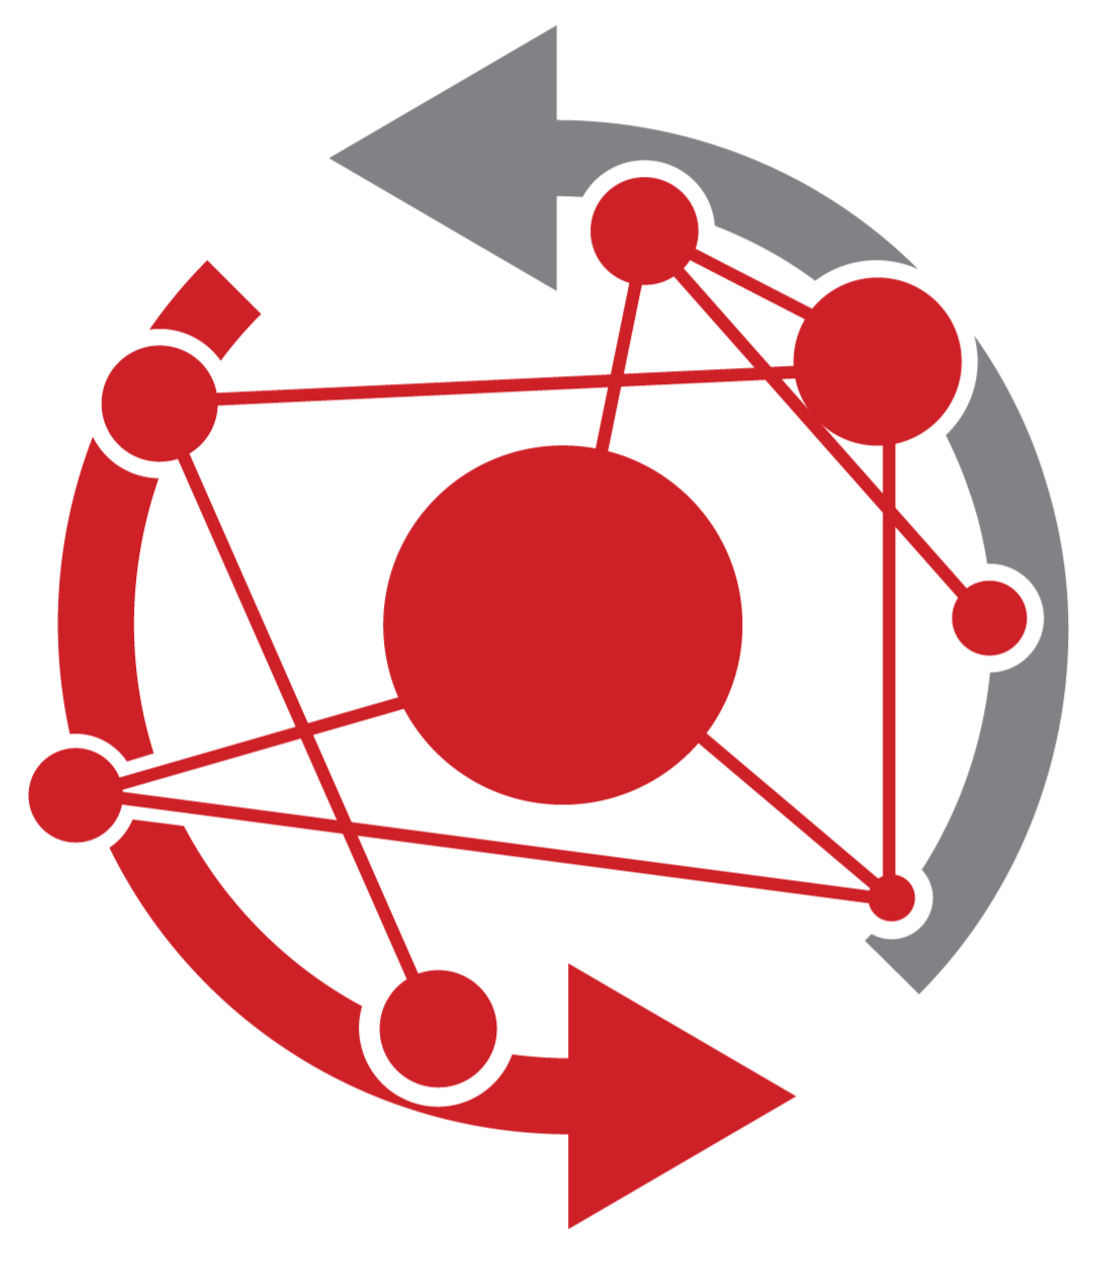
\includegraphics[scale=1]{Cover.png}
    \end{figure}
    \begin{center}    
      \small {
        Wersja \version -- \@date \\
        \vspace{0.3 cm}
        Tłumaczenie na język polski Michał Januszewski\\
        wersja tłumaczenia \translationver
      }
    \end{center}
    \vspace{2.5 cm}
    \begin{center}
      \footnotesize{
        ©2006-2022 Jeff Sutherland and Scrum Inc., All Rights Reserved\\
        Scrum@Scale is a~registered trademark of Scrum Inc.\\
        Released under Creative Commons 4.0 Attribution-Sharealike License
      }
    \end{center}
  \end{titlepage}%
}
\makeatother

\title{Przewodnik po Scrum@Scale}
\subtitle{Ostateczny Przewodnik po Scrum@Scale:\\ Skalowanie, które działa}
\author{}
\date{Luty 2022}
\newcommand{\version}{2.1}
\newcommand{\translationver}{2023.06.09}


\begin{document}
\maketitle
\tableofcontents
\subsection{Wstęp do Przewodnika po Scrum@Scale}\label{preface-to-the-ScrumatScale-guide}

Scrum, jak pierwotnie opisano w~przewodniku o~Scrumie, skupia się na tym, aby pojedynczy Scrum Team mógł dostarczyć optymalną wartość, utrzymując jednocześnie zrównoważone tempo pracy. Od momentu swojego powstania, Scrum jest wykorzystywany do tworzenia produktów, procesów i~usług, które wymagają zaangażowania kilku zespołów.

W praktyce wielokrotnie zaobserwowano, że wraz ze wzrostem liczby zespołów Scrum w~organizacji pojawiają się dwa główne problemy:


\begin{itemize}%[label={\huge\textbullet}]
\itemsep10pt
\item
  Wraz z~rosnącą liczbą zespołów, wolumen, szybkość i~jakość produktu ich pracy (działającego produktu) na zespół zaczęły spadać, z~powodu problemów takich jak zależności międzyzespołowe, powielanie pracy i~nadmiar komunikacji.
\item
 Oryginalna struktura zarządzania była nieskuteczna w~osiąganiu zwinności biznesowej. Pojawiły się problemy z~konkurującymi priorytetami oraz brakiem zdolności do szybkiego przesówania zespołów w~celu reagowania na dynamiczne warunki rynkowe.
\end{itemize}

Aby przeciwdziałać tym problemom, potrzebny był framework, który umożliwiłby skuteczne koordynowanie pracy wielu Scrum Teamów. Framework ten miałby na celu osiągnięcie następujących celów:

\begin{itemize}
\itemsep10pt
\item
  Liniowa skalowalność: Odpowiadający procentowy wzrost dostarczenia działającego produktu wraz ze wzrostem liczby zespołów
\item
 Zwinność biznesowa: Możliwość szybkiej reakcji na zmiany poprzez dostosowanie początkowej stabilnej konfiguracji
\end{itemize}

Scrum@Scale pomaga organizacji skupić wiele Sieci Scrum Teamów na priorytetowych celach. Celem jest osiągnięcie tego poprzez ustanowienie struktury, która naturalnie rozszerza sposób działania pojedynczego zespołu Scrum na Sieć, a~funkcja menedżerska istnieje w~ramach Minimum Viable Bureaucracy (MVB).

Sieć może osiągnąć liniową skalowalność, gdy jej cechy są niezależne od jej wielkości. Projektowanie i~koordynowanie Sieci Scrum Teamów w~tym celu nie ogranicza wzrostu w~określony sposób. Zamiast tego pozwala na organiczny wzrost Sieci, oparty na jej unikalnych potrzebach i~w zrównoważonym tempie zmian, które mogą być lepiej zaakceptowane przez zaangażowane osoby.

Minimalna wykonalna biurokracja jest definiowana jako posiadanie najmniejszej ilości organów zarządzających i~procesów potrzebnych do realizacji funkcji organizacji bez utrudniania dostarczania wartości dla klienta. Pomaga osiągnąć zwinność biznesową poprzez zmniejszenie opóźnienia decyzyjnego (czasu na podjęcie decyzji), co zostało odnotowane jako podstawowy czynnik sukcesu. Aby rozpocząć wdrażanie Scrum@Scale, konieczna jest znajomość Manifestu Agile oraz Przewodnika po Scrumie 2020. Niezrozumienie natury zwinności uniemożliwi jej osiągnięcie. Jeśli organizacja nie potrafi Scrum, nie może się skalować.


\subsection{Cel Przewodnika po Scrum@Scale}\label{purpose-of-the-ScrumatScale-guide}

Ten przewodnik dostarcza definicji Scrum@Scale oraz elementów jego ram. Wyjaśnia odpowiedzialności skalowanych ról, skalowanych zdarzeń i~artefaktów przed\-się\-bior\-stwa, a~także zasady, które je wiążą.

Przewodnik ten składa się z~czterech podstawowych sekcji:

\begin{itemize}
\itemsep1pt\parskip0pt\parsep0pt
\item
  wprowadzenia do Scrum@Scale, z~podstawami do rozpoczęcia pracy
\item
  przeglądu cyklu Scrum Mastera
\item
  przegląd cyklu Product Ownera
\item
  prezentacja łączenia cykli.
\end{itemize}

Każdy komponent służy konkretnemu celowi, który jest wymagany do osiągnięcia sukcesu w~skalowaniu. Zmiana ich podstawowej konstrukcji lub idei, pominięcie ich lub nieprzestrzeganie podstawowych zasad przedstawionych w~tym przewodniku ogra-ni-cza korzyści płynące ze Scrum@Scale.

Konkretne taktyki wykraczające poza podstawową strukturę i~zasady wdrażania każ\-de\-go komponentu różnią się i~nie są opisane w~tym przewodniku. Inne źródła dostarczają uzupełniających wzorców, procesów i~spostrzeżeń.

\subsection{Definicje}\label{definitions}

Scrum to lekki framework, który pomaga ludziom, zespołom i~organizacjom generować wartość poprzez adaptacyjne rozwiązania złożonych problemów.

Przewodnik po Scrum opisuje minimalny zestaw elementów, które tworzą środowisko Zespołu napędzające innowacyjność, zadowolenie klienta, wydajność i~szczęście. Scrum wykorzystuje radykalną przejrzystość i~serię formalnych wydarzeń, aby zapewnić możliwości kontroli i~adaptacji Zespołu i~jego produktu(ów).

Scrum@Scale to lekki framework organizacyjny, w~którym Sieć Zespołów działających zgodnie z~Przewonikiem po Scrumie może rozwiązywać złożone problemy adaptacyjne, a~jednocześnie kreatywnie dostarczać produkty o~jak najwyższej wartości. Te ,,produkty'' mogą być fizyczne, cyfrowe, złożone zintegrowane systemy, procesy, usługi itp.

Przewodnik po Scrum@Scale opisuje minimalny zbiór komponentów do skalowania Scrum poprzez zastosowanie Scruma i~wynikającej z~niego zwinności biznesowej w~całej organizacji. Może być stosowany we wszystkich rodzajach organizacji: w~przemyśle, rządzie, organizacjach non-profit lub w~środowisku akademickim. Jeśli organizacja nie korzysta jeszcze z~Scrum, będzie wymagała zmian w~swoim modelu operacyjnym.

W Scrumie dba się o~to, aby rozdzielić odpowiedzialność za ,,co'' (produkt) od ,,jak'' (procesu). Tą samą uwagę przywiązuje się do Scrum@Scale, tak aby kompetencje i~odpowiedzialność były wyraźnie zrozumiałe. Eliminuje to niepotrzebne konflikty organizacyjne, które uniemożliwiają zespołom osiągnięcie optymalnej produktywności. Ponieważ Scrum@Scale składa się z~komponentów, umożliwia organizacji dos\-to\-so\-wa\-nie strategii transformacji i~implementacji do swoich potrzeb. Daje to organizacji możliwość stopniowego ukierunkowania wysiłków na rzecz zmian w~obszarach uznanych za najbardziej wartościowe lub wymagające adaptacji, a~następnie przechodzenia do innych.

Scrum@Scale dzieli te składniki na dwa cykle: cykl Scrum Mastera (,,jak'') i~cykl Product Ownera (,,co''), które przecinają się na dwóch elementach i~dzielą z~trzecim. Cykle te, traktowane jako całość, tworzą potężną strukturę wspierającą koordynację wysiłków wielu zespołów wzdłuż jednej ścieżki.

\subsection{Komponenty Scrum@Scale}\label{the-components-of-scrumatscale}
\begin{figure}[H]
    \centering
    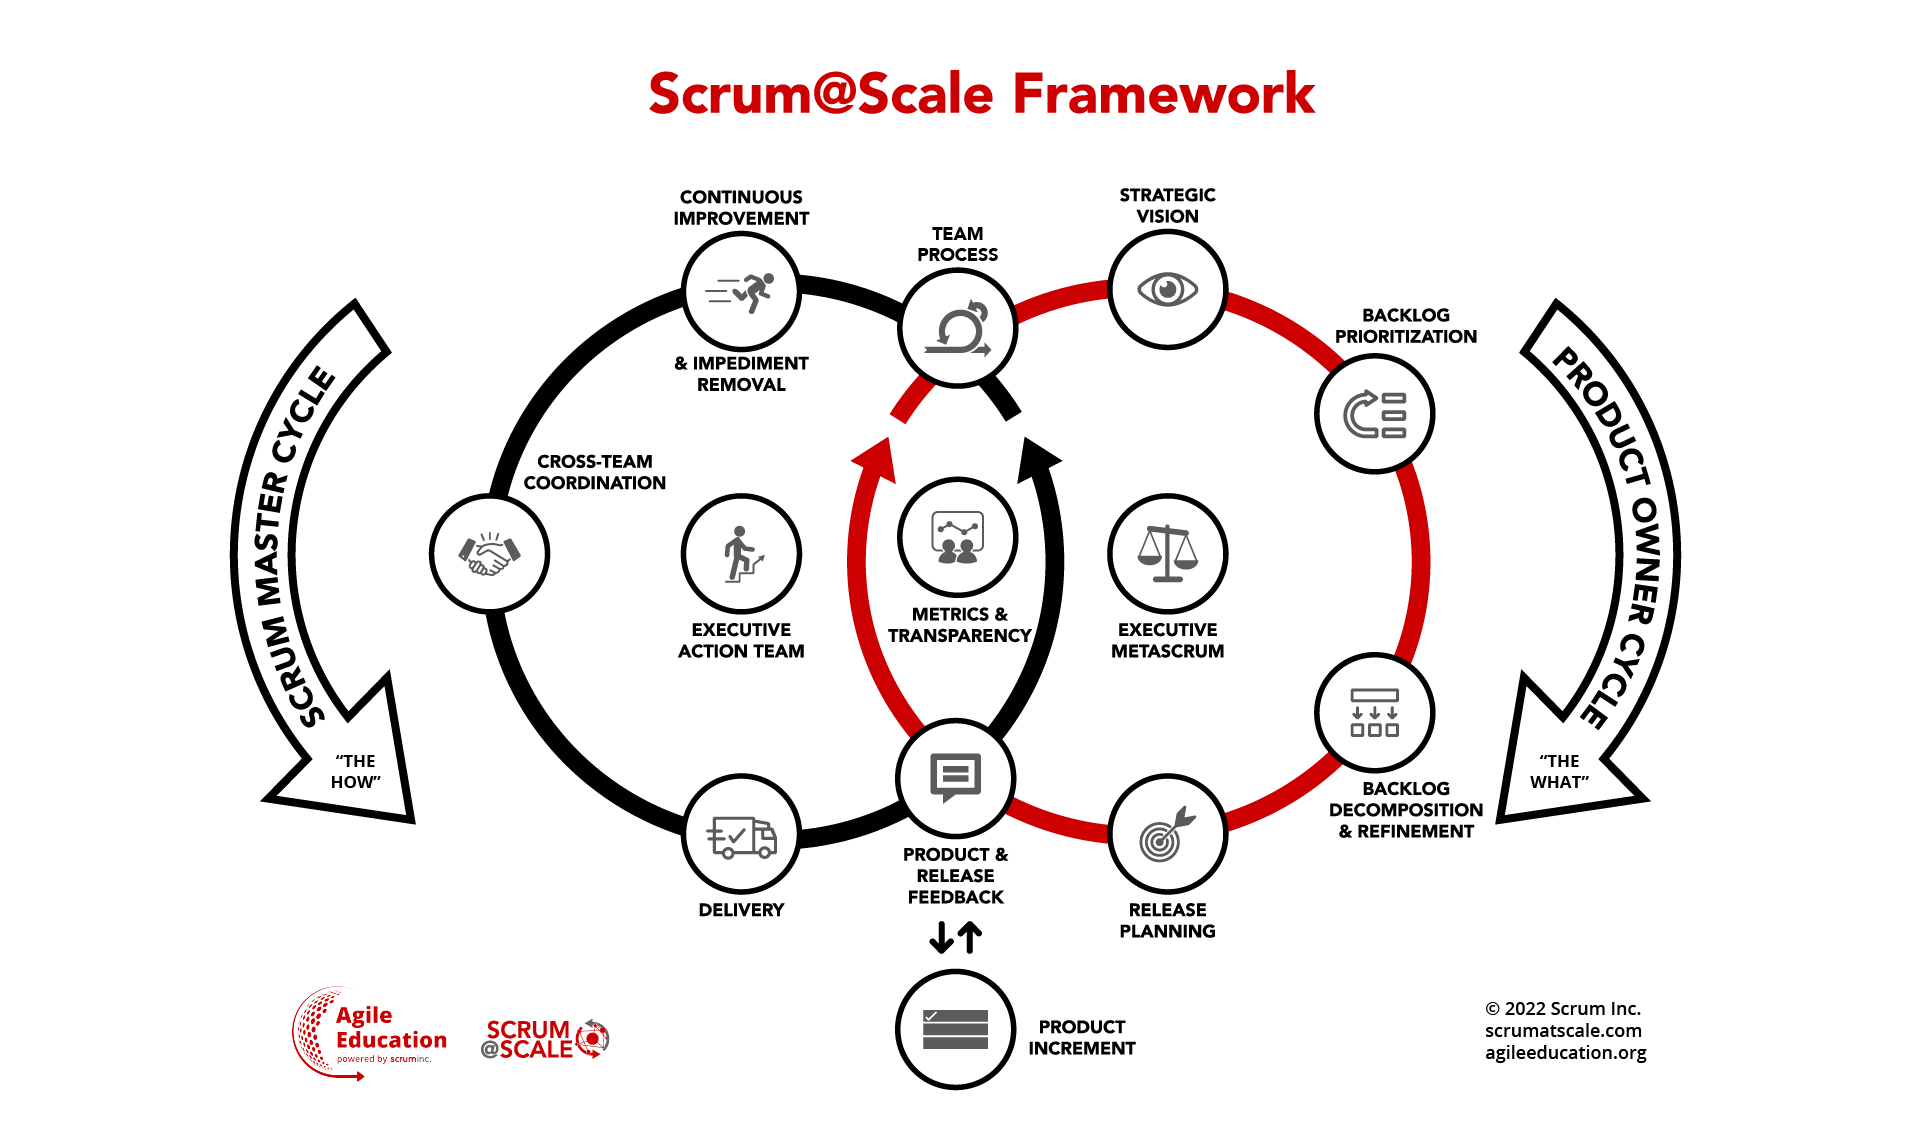
\includegraphics[scale=0.25]{SMPO-Cycle.png}
\end{figure}

\subsubsection{Kultura Oparta na Wartościach}\label{values-driven-culture}

Scrum@Scale ma na celu zbudowanie zdrowej kultury organizacyjnej poprzez filary empirycznej kontroli procesu i~Wartości Scrum. Filary empirycznej kontroli procesu to transparencja, inspekcja i~adaptacja. Te filary są realizowane przez Wartości Scrum: Otwartość, Odwagę, Skupienie, Szacunek i~Zaangażowanie.

Otwartość wspiera transparencję w~całej pracy i~wszystkich procesach, a~bez niej nie ma możliwości uczciwej inspekcji i~próby adaptacji. Odwaga odnosi się do podejmowania odważnych skoków wymaganych do szybszego dostarczania wartości w~innowacyjny sposób. Skupienie i~Zaangażowanie odnoszą się do sposobu, w~jaki podchodzimy do naszych obowiązków, stawiając dostarczanie wartości dla klienta na pierwszym miejscu. Wreszcie, wszystko to musi mieć miejsce w~środowisku opartym na Szacunku dla ludzi wykonujących pracę, bez których nic nie może powstać.

Scrum@Scale pomaga organizacjom rozwijać się poprzez wspieranie pozytywnego środowiska uczenia się zespołu, pracującego w~zrównoważonym tempie i~stawiającego wartość dla klienta na czele.

\subsubsection{Rozpoczęcie pracy: Wprowadzenie Agile Operating
System}\label{getting-started-installing-an-agile-operating-system}

Podczas wdrażania sieci zespołów, krytycznym jest opracowanie skalowalnego Modelu Referencyjnego przed skalowaniem. Model Referencyjny to mały zestaw zespołów, które koordynują swoje działania, aby zrealizować każdy Sprint. Gdy te zespoły z~powodzeniem wdrażają Scrum, reszta organizacji ma funkcjonujący, zdrowy przykład Scrum do powielenia. Służy on jako prototyp do skalowania Scrum w~kolejnej sieci zespołów. Wszelkie braki w~implementacji Scrum zostaną spotęgowane, gdy wdrożonych zostanie wiele zespołów. Problemy ze skalowaniem obejmują polityki i~procedury organizacyjne lub praktyki rozwojowe, które blokują wydajność i~frustrują zespoły.

W przypadku skalowania, Model Referencyjny najlepiej sprawdza się poprzez grupowanie zespołów, które muszą koordynować swoje działania, aby dostarczyć w~pełni zintegrowany zestaw Incrementów w~ramach Scrum of Scrums (SoS). Aby działać efektywnie, Scrum of Scrums musi być wspierane przez minimalną wykonalną biurokrację składającą się z~dwóch grup przywódczych: forum Executive MetaScrum (EMS), skoncentrowanego na tym, co jest produkowane przez Scrum of Scrums oraz Executive Action Team (EAT) skoncentrowanego na tym, jak mogą to zrobić szybciej. Komponenty Executive MetaScrum i~Executive Action Team są węzłami, wokół których obraca się każdy cykl.

\subsubsection{Skalowanie Zespołów}\label{scaling-the-teams}

W Scrumie idealnym stanem jest, aby Scrum Team był niezależną ścieżką do produkcji. Jako taki potrzebuje członków, którzy mają wszystkie umiejętności niezbędne do przejścia od ideacji do wdrożenia. Scrum of Scrums to większy zespół złożony z~wielu zespołów, który replikuje ten ideał w~skali. Każdy zespół w~ramach Scrum of Scrums musi wypełniać elementy Team Process.

\subsubsection{Team Process}\label{the-team-process}

Team Process to Scrum zgodnie z~zaleceniami Przewodnika po Scrum. Ponieważ każdy Scrum Team posiada Product Ownera i~Scrum Mastera, stanowi on pierwsze skrzyżowanie cykli Product Ownera i~Scrum Mastera. Celami Team Process są:
\begin{itemize}
\itemsep1pt\parskip0pt\parsep0pt
\item
 Zmaksymalizowanie przepływu ukończonej pracy, która spełnia Definition\ of\ Done
\item
  Zwiększanie wydajności zespołu w~czasie
\item
  Działać w~sposób, który jest trwały i~wzbogaca zespół
\item
  Przyspieszyć pętlę feedbacku od klienta
\end{itemize}

\subsubsection{Scrum of Scrums (SoS)}\label{the-scrum-of-scrums}

Scrum of Scrums działa tak, jakby był Scrum Teamem, spełniając elementy Team Process ze skalowanymi wersjami odpowiedzialności Scrum, wydarzeń i~artefaktów. Podczas gdy Przewodnik po Scrum definiuje optymalną wielkość zespołu jako mniejszą niż 10 osób, Harvard research\textsuperscript{\hyperref[citation4]{4}} ustalił, że optymalna wielkość zespołu to 4,6 osoby (średnio). Dlatego optymalna liczba zespołów w~Scrum of Scrums to 4 lub 5.

Jako dynamiczna grupa, zespoły tworzące Scrum of Scrums są odpowiedzialne za w~pełni zintegrowany zestaw potencjalnie nadających się do dostarczenia Incrementów produktu na koniec każdego Sprintu. Optymalnie, realizują one wszystkie funkcje wymagane do wydania wartości bezpośrednio klientom.

\begin{figure}[H]
    \centering
    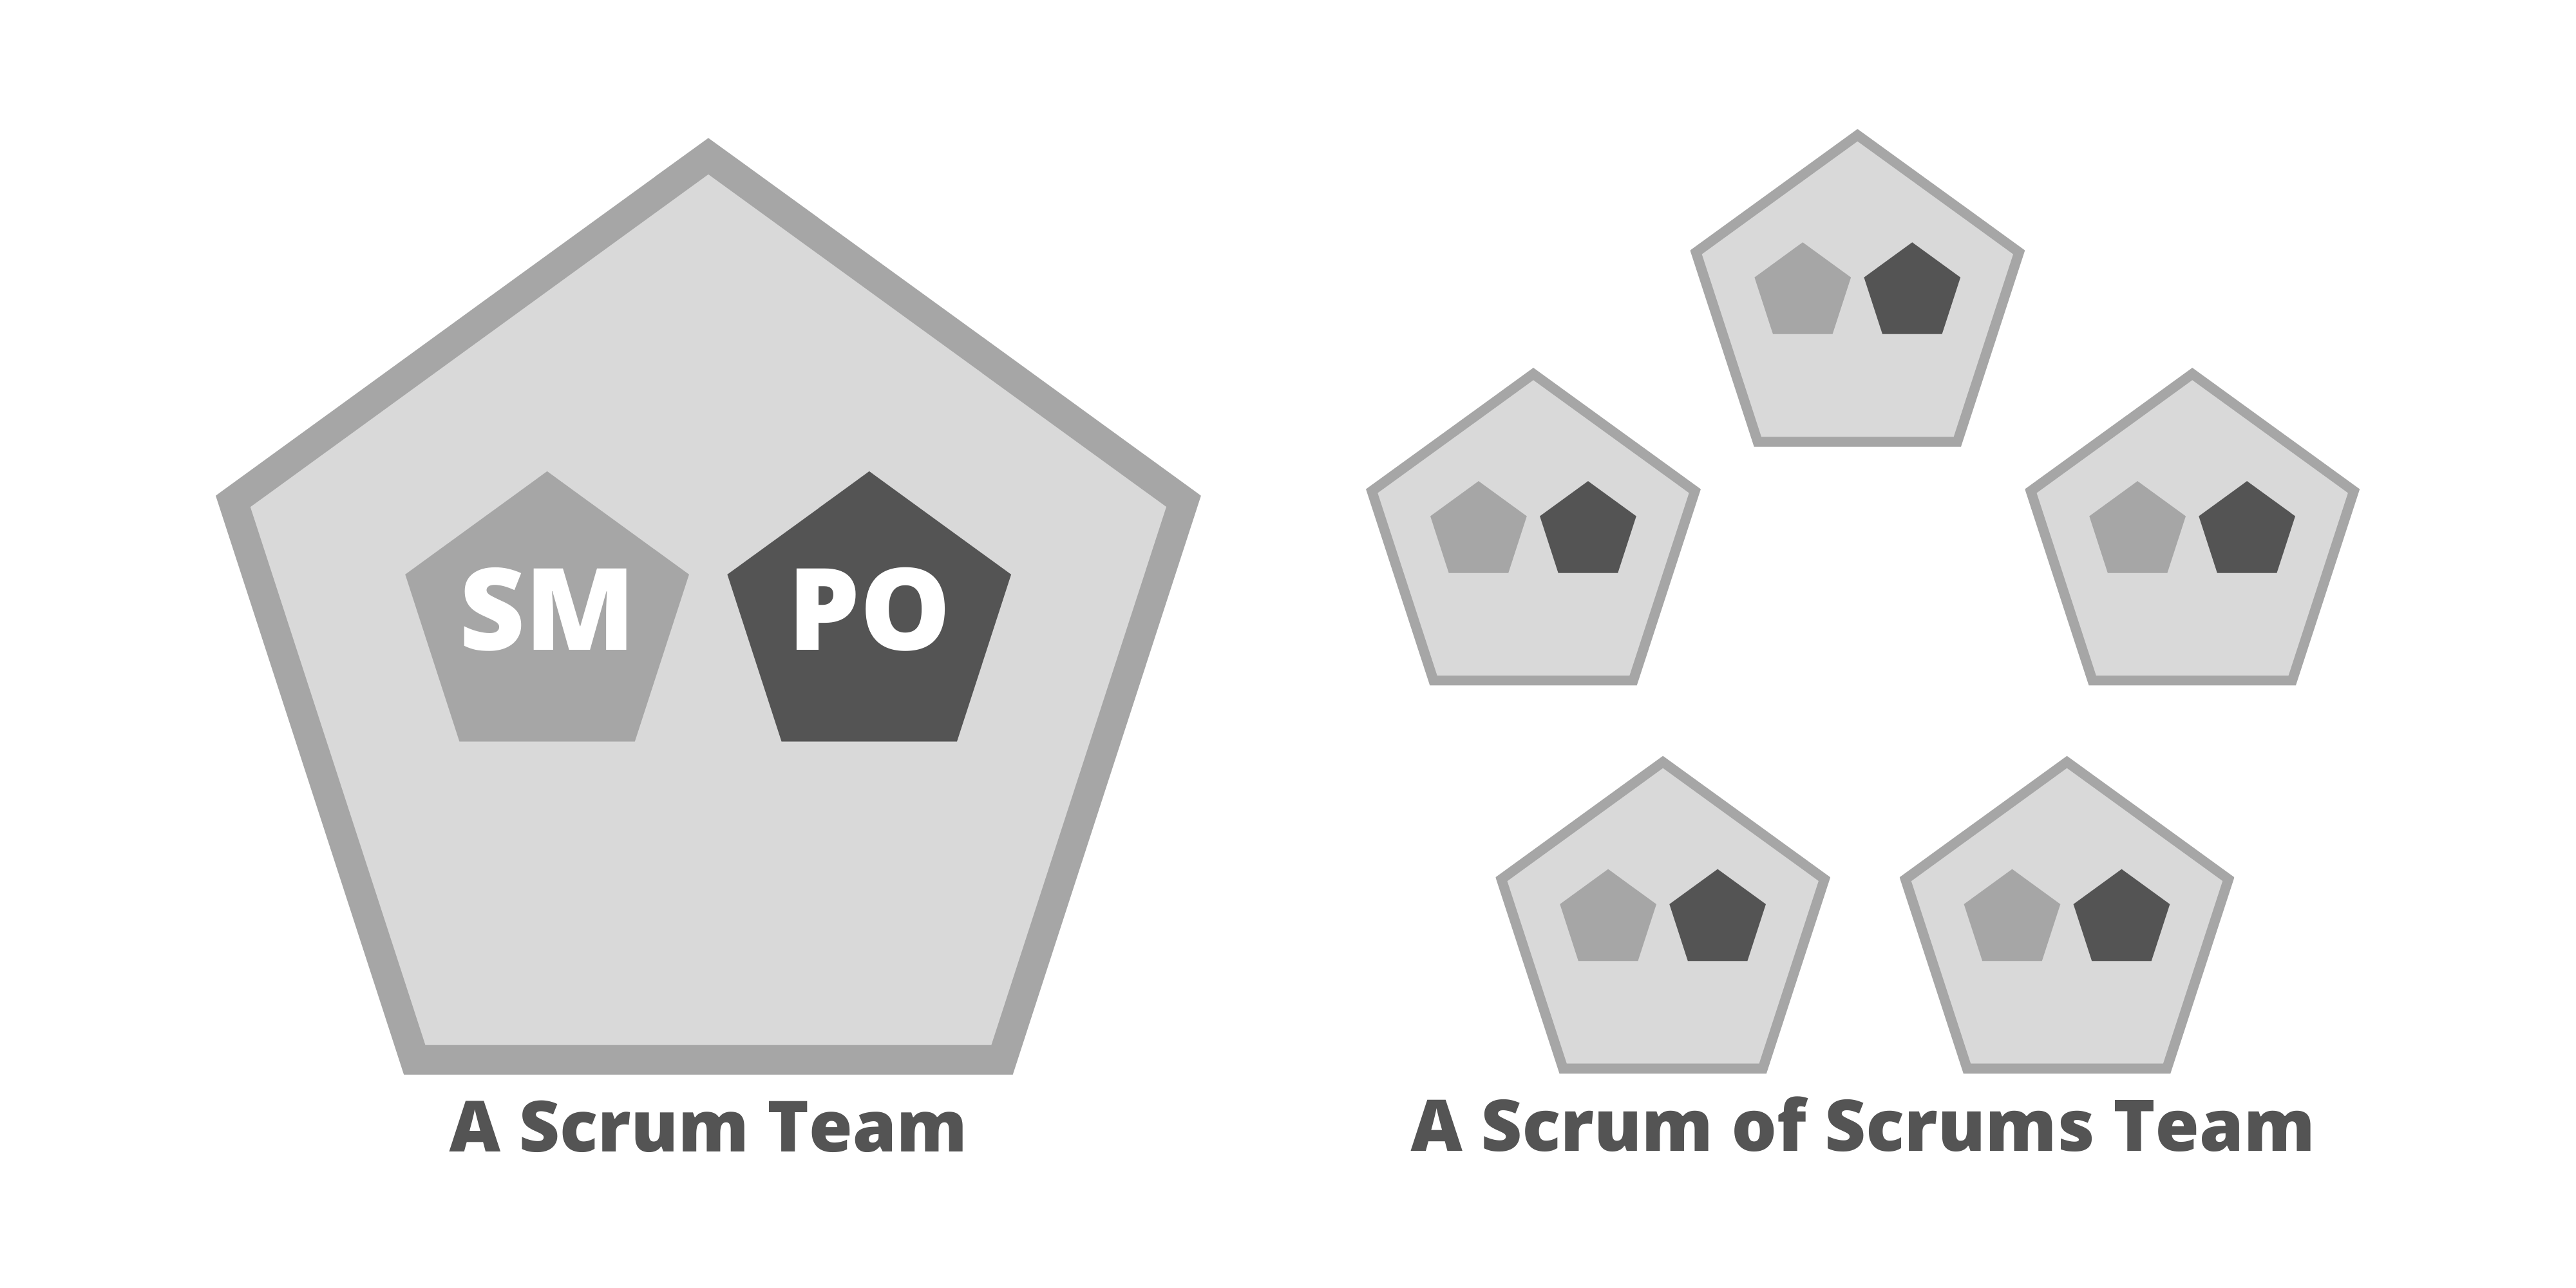
\includegraphics[scale=0.15]{1.png}
\end{figure}

\emph{UWAGA: Na powyższym i~poniższych schematach, jasnoszare obrysowane pięciokąty reprezentują zespół. Tam, gdzie ma to zastosowanie, zdecydowaliśmy się przedstawić SM i~PO jako mniejsze pięciokąty. Diagramy te mają być jedynie przykładami, ponieważ każdy schemat organizacyjny może się znacznie różnić.}

\subsubsection{Skalowanie w~więszych organizacjach}\label{scaling-in-larger-organizations}

W zależności od wielkości wdrożenia, może być potrzebnych więcej niż jedno Scrum of Scrums do dostarczenia złożonego produktu. w~takich przypadkach można utworzyć Scrum of Scrum of Scrums (SoSoS) z~kilku Scrum of Scrums. Każde z~nich będzie miało skalowane wersje ról, artefaktów i~wydarzeń każdego Scrum of Scrums.

Skalowanie Scrum of Scrums zmniejsza liczbę ścieżek komunikacyjnych w~organizacji, dzięki czemu złożoność obciążenia komunikacyjnego jest ograniczona. SoSoS współpracuje z~Scrum of Scrums dokładnie w~ten sam sposób, w~jaki Scrum of Scrums współpracuje z~pojedynczym zespołem Scrum, co pozwala na liniową skalowalność.

\begin{figure}[H]
    \centering
    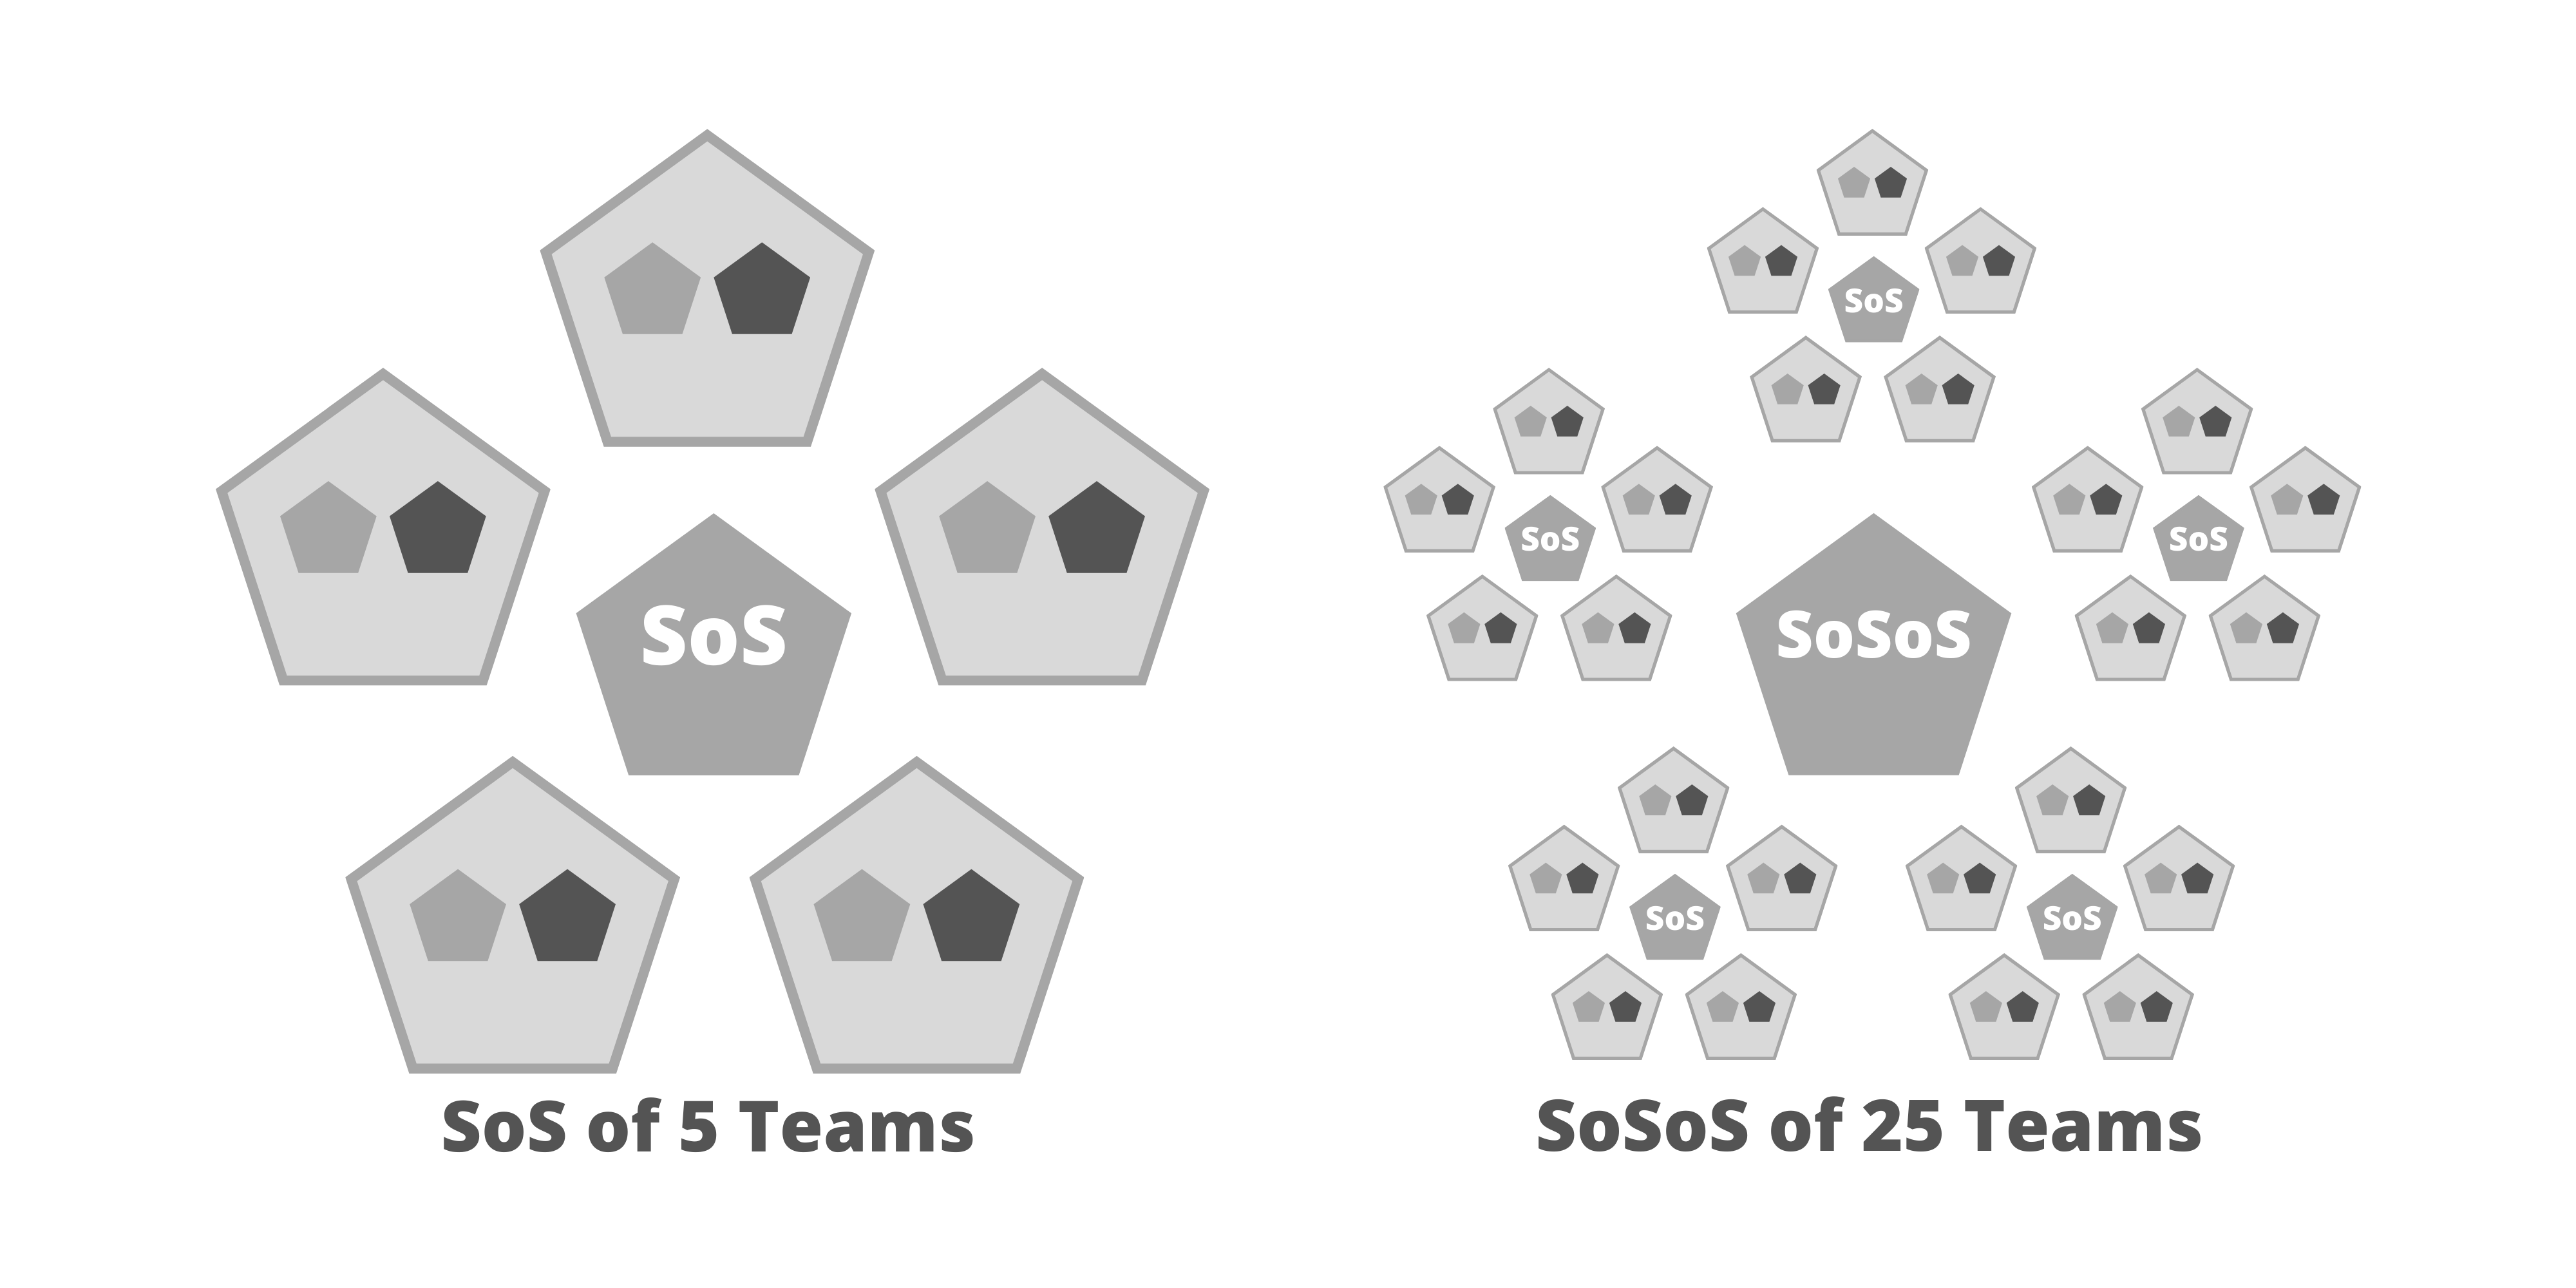
\includegraphics[scale=0.15]{2.png}
\end{figure}

\emph{UWAGA: w~celu uproszczenia, liczby zespołów i~grup w~przykładowych diagramach są symetryczne. Mają one jedynie charakter przykładowy, ponieważ każdy diagram organizacyjny może znacznie się różnić.}

\subsubsection{Skalowanie Wydarzeń i~Ról}\label{scaling-the-events-and-roles}

Jeśli Scrum of Scrums (SoS) działa jak Scrum Team, to musi skalować wydarzenia Scrum i~odpowiadające im odpowiedzialności zespołów. Aby koordynować ,,jak'' w~każdym sprincie, SoS będzie musiał przeprowadzać skalowane wersje Daily Scrum i~Sprint Retrospective. Aby koordynować ,,co'' w~każdym sprincie, SoS będzie musiał przeprowadzać skalowane wersje Sprint Planning i~Sprint Review. Jako praktyka ciągła, wymagane będzie także skalowanie Backlog Refinement.

Skalowane wersje Daily Scrum i~Sprint Retrospective są prowadzone przez Scrum Mastera dla grupy, nazywanego Scrum of Scrums Master (SoSM). Skalowane wersje Sprint Review i~Backlog Refinementu prowadzone są przez Product Owners Team (PO Team) pod kierownictwem Chief Product Owner (CPO). Skalowana wersja Sprint Planningu odbywa się z~zespołem Product Ownerów i~ze Scrum Masterami. Product Owners Team zdobywa wgląd w~to, co zostanie dostarczone w~bieżącym Sprincie, a~Scrum Masterzy zdobywają wgląd w~zdolność produkcyjną i~techniczną. Role Scrum of Scrums Mastera i~Chief Product Ownera skalują się w~grupy liderów, które następnie prowadzą swoje odpowiadające im cykle, zgodnie z~komponentami Scrum@Scale.

\subsubsection{Wydarzenie: Scaled Daily Scrum (SDS)}\label{event-the-scaled-daily-scrum}

Głównymi punktami Daily Scrum są postępy w~realizacji Celu Sprintu oraz prze\-szko\-dy w~realizacji tego zobowiązania. w~środowisku skalowanym Scrum\ of\ Scrums musi rozumieć zbiorowy postęp i~reagować na przeszkody zgłaszane przez uczestniczące zespoły; dlatego w~Scaled Daily Scrum (SDS) uczestniczy co najmniej jeden przedstawiciel z~każdego zespołu. Może uczestniczyć w~nim dowolna osoba lub grupa osób z~uczestniczących zespołów, w~miarę potrzeb.

Aby zoptymalizować współpracę i~wydajność, wydarzenie Scaled Daily Scrum odzwierciedla Daily Scrum, w~tym, że:

\begin{itemize}
\itemsep1pt\parskip0pt\parsep0pt
\item
  Jest ograniczony czasowo do 15 minut lub mniej
\item
  Musi w~nim uczestniczyć przedstawiciel każdego zespołu.
\item
  Jest miejscem, gdzie można dyskutować o~tym, jak zespoły mogą pracować ze sobą bardziej efektywnie, co zostało zrobione, co zostanie zrobione, co idzie źle i~dlaczego, oraz co grupa ma zamiar z~tym zrobić.
\end{itemize}

Kilka przykładowych pytań do zadania:

\begin{itemize}
\itemsep1pt\parskip0pt\parsep0pt
\item
  Jakie przeszkody ma zespół, które uniemożliwią mu osiągnięcie Celu Sprintu lub które wpłyną na zaplanowane dostarczanie.
\item
  Czy zespół robi coś, co uniemożliwi innemu zespołowi osiągnięcie jego Celu Sprintu lub co wpłynie na jego zaplanowane dostarczanie.
\item
  Czy odkryto jakieś nowe zależności między zespołami lub sposób rozwiązania istniejącej zależności?
\end{itemize}

\subsubsection{Wydarzenie: Scaled Retrospective}\label{event-the-scaled-retrospective}

Co każdym Sprint, Scrum of Scrums organizuje przeskalowaną wersję Sprint Retrospective, podczas której Scrum Masterzy każdego zespołu spotykają się i~omawiają, jakie eksperymenty zostały przeprowadzone w~celu ciągłego doskonalenia oraz ich wyniki. Ponadto, powinni omówić następną rundę eksperymentów oraz to, jak udane usprawnienia mogą być wykorzystane przez grupę zespołów lub poza nią.

\subsection{Scrum Master Cycle: Koordynacja ,,Jak''}\label{the-scrum-master-cycle}

\subsubsection{Rola: Scrum of Scrums Master (SoSM)}\label{role-the-scrum-of-scrums-master}
Scrum Master w~Scrum of Scrum nazywany jest Scrum of Scrum Master (SoSM). Scrum of Scrums Master jest odpowiedzialny za zapewnienie, że wydarzenia skalowane odbywają się, są produktywne, pozytywne i~utrzymane w~ramach czasowych. Scrum of Scrums Master może być jednym z~Scrum Masterów zespołu lub osobą specjalnie dedykowaną do tej roli. Są oni odpowiedzialni za wydawanie połączonych efektów pracy zespołów oraz ciągłe podnoszenie efektywności Scrum of Scrums. Dotyczy to większej przepustowości zespołu, niższych kosztów i~wyższej jakości. Aby osiągnąć te cele, muszą:

\begin{itemize}
\itemsep1pt\parskip0pt\parsep0pt
\item
  Blisko współpracować z~Chief Product Ownerem, aby dostarczyć Increment produktu, który potencjalnie można wydać, przynajmniej w~każdym sprincie
\item
  Koordynacja dostarczania produktów przez zespoły z~planami wydań zespołu Product Ownerów
\item
  Uwidacznianie przeszkód, usprawnień procesu i~postępów w~organizacji
\item
  Ułatwiają ustalanie priorytetów i~usuwanie przeszkód, zwracając szczególną uwa\-gę na zależności między zespołami
\end{itemize}

Scrum of Scrums Master jest prawdziwym liderem, który służy zespołom i~organizacji poprzez zrozumienie zależności międzyzespołowych, w~tym poza Scrum of Scrums oraz umożliwienie koordynacji i~komunikacji międzyzespołowej. Są odpowiedzialni za informowanie Chief Product Ownera, interesariuszy i~szerszej części organizacji poprzez przekazywanie informacji o~postępach w~rozwoju produktu, statusie usuwania przeszkód i~innych metrykach. Scrum of Scrums Master prowadzi przez przykład, mentorując innych w~celu zwiększenia efektywności i~przyjęcia Scruma w~całej organizacji.

W przypadku, gdy wiele Scrum of Scrumów jest zgrupowanych w~Scrum of Scrum of Scrum, wtedy potrzebny jest Scrum of Scrum of Scrum Master (SoSoSM), aby koordynować z~tej szerszej perspektywy.

\subsubsection{Centrum cyklu Scrum Mastera: Executive Action Team (EAT)}\label{the-hub-of-the-sm-cycle}

Executive Action Team (EAT) wypełnia obowiązki Scrum Mastera dla całej organizacji agile. Ten zespół liderski tworzy ekosystem agile, który umożliwia optymalne funkcjonowanie Modelu Referencyjnego, poprzez:

\begin{itemize}
\itemsep1pt\parskip0pt\parsep0pt
\item
  wdrażanie wartości Scrum
\item
  dbanie o~to, aby role Scrumowe były tworzone i~wspierane
\item
  wydarzenia Scrumowe są organizowane i~uczestniczone
\item
  Artefakty Scrum i~związane z~nimi zobowiązania są generowane, poddawane transparencji i~aktualizowane w~trakcie każdego Sprintu.
\item
 formułowanie wytycznych i~procedur, które pełnią rolę warstwy translacyjnej pomiędzy Modelem Referencyjnym a~każdą częścią organizacji, która nie jest zwinna.
\end{itemize}

Executive Action Team jest odpowiedzialny za usuwanie przeszkód, których nie mogą usunąć członkowie Scrum of Scrums (lub szerszej sieci). Dlatego musi składać się z~osób, które są upoważnione, politycznie i~finansowo, do ich usunięcia. Funkcją Executive Action Team jest koordynacja wielu Scrum of Scrums (lub szerszych sieci) oraz interfejs z~wszelkimi nieagile'owymi częściami organizacji. Jak każdy Scrum Team potrzebuje Product Ownera, Scrum Mastera i~przejrzystego backlogu.

\begin{figure}[H]
    \centering
    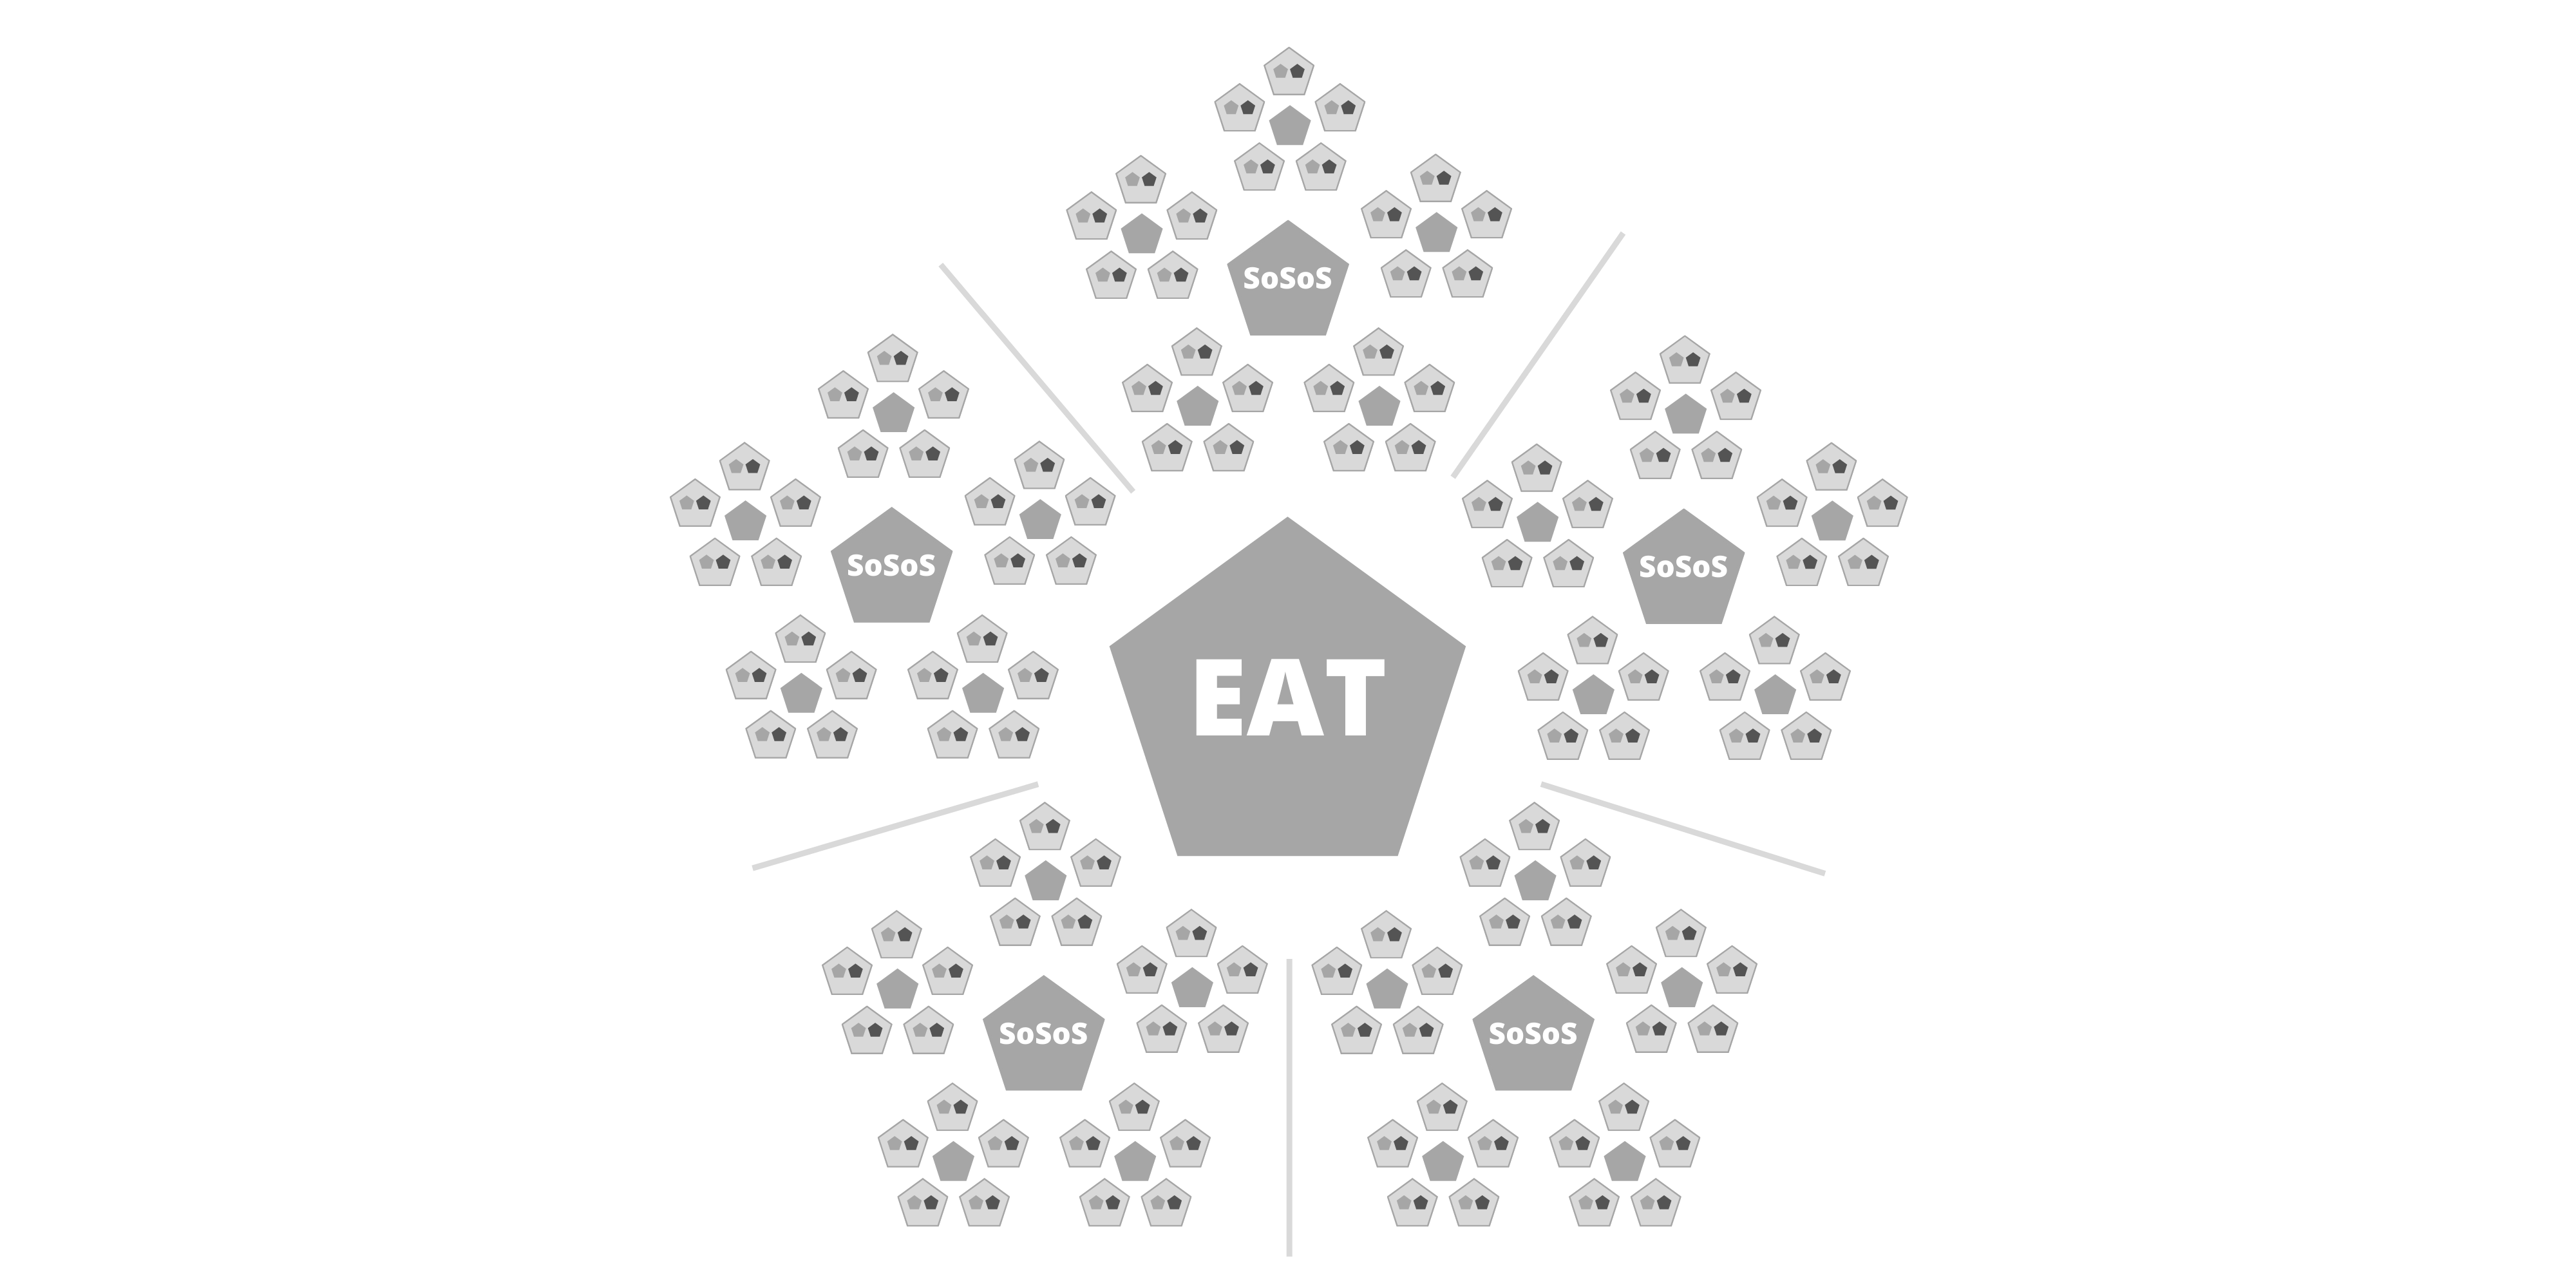
\includegraphics[scale=0.15]{3.png}
    
\end{figure}


\emph{Przykładowy schemat przedstawiający EAT koordynujący 5 grup po 25 zespołów}

\subsubsection{EAT Backlog i~odpowiedzialności}\label{EAT-backlog-and-responsibilities}

Produktem Executive Action Team (EAT) jest stworzenie systemu operacyjnego Agile dla organizacji. EAT tworzy Product Backlog składający się z~inicjatyw służących ciągłej transformacji organizacji w~celu osiągnięcia celu, jakim jest większa zwinność biznesowa. Backlog ten obejmuje również usprawnienia procesów, które usuwają przeszkody oraz takie, które wymagają standaryzacji.

Do obowiązków Executive Action Team należą m.in.:

\begin{itemize}
\itemsep1pt\parskip0pt\parsep0pt
\item
  Stworzenie zwinnego systemu operacyjnego dla Modelu Referencyjnego w~mia\-rę jego skalowania w~organizacji, w~tym korporacyjnych zasad operacyjnych, procedur i~wytycznych umożliwiających zwinność
\item
 Zapewnienie stworzenia, finansowania i~wsparcia organizacji Product Ownerów
\item
  Pomiar i~poprawa jakości Scruma w~organizacji
\item
  Budowanie zdolności w~organizacji do zwinności biznesowej
\item
  Stworzenie centrum ciągłego uczenia się dla profesjonalistów Scruma
\item
  Wspieranie poszukiwania nowych sposobów pracy
\end{itemize}

Funkcją Executive Action Team jest dopilnowanie, aby te backlog został zrealizowany. Mogą to zrobić sami lub umocować do tego inną grupę. Ponieważ Executive Action Team jest odpowiedzialny za jakość Scruma w~organizacji, raportuje do niego cała organizacja Scrum Masterów.

Organizacja Scrum Master (Scrum Masters, Scrum of Scrum Masters oraz Executive Action Team) pracują jako całość, aby wdrożyć komponenty Cyklu Scrum Mastera. Te unikalne komponenty to:


\begin{itemize}
\itemsep1pt\parskip0pt\parsep0pt
\item
  ciągłe doskonalenie i~usuwanie przeszkód
\item
  Koordynacja pomiędzy zespołami
\item
  Dostarczanie
\end{itemize}

\subsubsection{Ciągłe doskonalenie i~usuwanie przeszkód}\label{Continuous-improvement-and-impediment-removal}

Najlepiej byłoby, gdyby przeszkody zostały usunięte tak szybko, jak to możliwe. Jest to krytyczne, aby uniknąć skalowania samych przeszkód oraz dlatego, że te nierozwiązane mogą spowolnić produktywność. Dlatego celami ciągłego doskonalenia i~usuwania przeszkód

\begin{itemize}
\itemsep1pt\parskip0pt\parsep0pt
\item
  zidentyfikowanie przeszkód i~przeformułowanie ich na możliwości poprawy
\item
  zapewnienie transparencji i~widoczności w~organizacji w~celu wprowadzania zmian
\item
  utrzymanie skutecznego środowiska do ustalania priorytetów i~usuwania przeszkód
\item
  sprawdzić, czy usprawnienia wpłynęły pozytywnie na metryki zespołu i/lub produktu
\end{itemize}

\subsubsection{Koordynacja pomiędzy zespołami}\label{cross-team-coordination}

Gdy do stworzenia wspólnego produktu potrzeba wielu zespołów,
usprawniona współpraca jest wymagana dla osiągnięcia sukcesu. Dlatego celami koordynacji między zespołami są:

\begin{itemize}
\itemsep1pt\parskip0pt\parsep0pt
\item
  synchronizacja podobnych procesów w~wielu powiązanych zespołach
\item
  ograniczanie zależności między zespołami, aby zapewnić, że nie staną się one przeszkodami
\item
  utrzymanie zgodności norm i~wytycznych zespołu w~celu uzyskania spójnych wyników
\end{itemize}

\subsubsection{Dostarczanie}\label{Delivery}

Ponieważ celem Scrum of Scrums jest funkcjonowanie jako jedna jednostka i~wspólne wydawanie, sposób dostarczania produktu wchodzi w~zakres ich działań jako grupy. Product Owners Team określa zarówno zawartość wydania, jak i~optymalny czas dostarczenia Incrementu do klientów.  Dlatego też celami dostarczania dla Scrum of Scrums są:

\begin{itemize}
\itemsep1pt\parskip0pt\parsep0pt
\item
  dostarczenie spójnego przepływu wartościowego produktu końcowego do klientów
\item
  zintegrowanie pracy różnych zespołów w~jeden spójny produkt
\item
  zapewnienie wysokiej jakości wrażeń klienta
\end{itemize}

\subsection{Cykl Product Ownera: Koordynacja ,,Co''}\label{The-product-owner-cycle}

\subsubsection{Skalowanie Product Ownera - Cykl Product Ownera}\label{Scaling-the-product-owner}

Dla każdego Scrum of Scrums istnieje wspólny backlog, który zasila sieć zespołów. Wymaga to Product Owners Team (PO Team), w~tym Chief Product Ownera, który jest odpowiedzialny jako Product Owner dla grupy zespołów. Głównym zadaniem PO Team jest zapewnienie, że priorytety poszczególnych zespołów podążają w~jednym kierunku. Umożliwia to koordynację backlogów poszczególnych zespołów oraz budowanie zgodności z~interesariuszami i~potrzebami klienta.

Product Owner każdego zespołu jest odpowiedzialny za kompozycję i~priorytetyzację Sprint Backlogu swojego zespołu i~może czerpać elementy ze wspólnego backlogu lub generować niezależne elementy backlogu według własnego uznania, tak jak jest to potrzebne do realizacji celów biznesowych.

Do głównych funkcji Product Owners Team należą:

\begin{itemize}
\itemsep1pt\parskip0pt\parsep0pt
\item
  komunikowanie nadrzędnej wizji produktu i~uczynienie jej widoczną dla wszystkich w~organizacji
\item
  budowanie współpracy z~kluczowymi interesariuszami w~celu zapewnienia wsparcia przy implementacji backlogu
\item
  stworzenie pojedynczego, zpriorytetyzowanego backlogu; upewnienie się, że unikamy duplikacji pracy
\item
  współpraca z~Scrum of Scrum Masterem w~celu stworzenia minimalnej, jednolitej ,,Definition of Done'', która dotyczy wszystkich zespołów
\item
  eliminowanie zależności zgłaszanych przez zespoły
\item
  wytworzenie skoordynowanej Roadmapy i~Release Planu
\item
  monitorowanie metryk, które dają obraz produktu i~rynku
\end{itemize}

\subsubsection{Rola: Chief Product Owner (CPO)}\label{role-the-chief-product-owner}

Chief Product Owner koordynuje priorytety z~zespołem Product Owners Team. Wspólnie dopasowują priorytety backlogu do potrzeb interesariuszy i~klientów. CPO może być indywidualnym Product Ownerem zespołu, który również pełni tę rolę, lub może być osobą specjalnie do tego przeznaczoną. Jego główne obowiązki są takie same, jak zwykłego Product Ownera, tylko że w~większej skali:

\begin{itemize}
\itemsep1pt\parskip0pt\parsep0pt
\item
  Wyznaczanie strategicznej wizji dla całego produktu
\item
  Tworzenie jednego, zpriorytetowego backlogu, który będzie dostarczany przez wszystkie zespoły
\item
  Podejmowanie decyzji, które metryki będzie monitorował Product Owners Team
\item
  Ocenianie feedbacku o~produkcie od klientów i~dostosowywanie do tych informacji wspólnego backlogu
\item
  Facylitacja wydarzenia MetaScrum (patrz poniżej)
\end{itemize}

Chief Product Owner jest odpowiedzialny wraz z~towarzyszącymi mu Scrum of Scrum Masterami za efektywne dostarczanie Incrementów produktu zgodnie z~Release Planem.

\subsubsection{Skalowanie Product Owners Team}\label{scaling-the-product-owner-team}

Posiadanie Product Owners Teamów umożliwia stworzenie sieci Product Ownerów, która skaluje się wraz z~ich powiązanym Scrum of Scrum. Nie ma konkretnego określenia związanego z~tymi rozszerzonymi jednostkami, a~ich Chief Product Ownerowie nie mają konkretnych, rozszerzonych tytułów. Każda organizacja jest zachęcana do opracowania własnych.

\subsubsection{Centrum cyklu PO: Executive MetaScrum (EMS)}\label{the-hub-of-the-po-cycle}

Aby pełnić rolę Product Ownera dla całej zwinnej organizacji, Chief Product Owner spotyka się z~kadrą zarządzającą i~kluczowymi interesariuszami podczas wydarzenia Executive MetaScrum. Wydarzenie to wywodzi się z~wzorca MetaScrum\textsuperscript{\ref{5}}. Jest to forum dla Liderów i~innych interesariuszy do wyrażania swoich preferencji dla PO Team, negocjowania priorytetów, dokonywania zmian w~budżecie lub zmiany składu zespołów w~celu zmaksymalizowania dostarczania wartości. w~żadnym innym momencie Sprintu decyzje te nie powinny być podejmowane.

Na Executive MetaScrum aktywna grupa liderów ustala wizję organizacyjną i~strategiczne priorytety, zestrajając wszystkie zespoły wokół wspólnych celów. Aby spotkanie to było efektywne, Chief Product Owner je facylituje, a~Product Owner każdego zespołu (lub jego pełnomocnik) musi w~nim uczestniczyć. To wydarzenie ma miejsce tak często, jak to jest potrzebne - przynajmniej raz na Sprint - aby zapewnić zgrany backlog w~ramach Scrum of Scrums.~ Optymalnie, ta grupa liderów działa jako Scrum Team.

W przypadku większych implementacji, gdzie istnieje wiele Scrum of Scrumów, może istnieć wiele MetaScrumów, które mają swój Strategic Backlog tworzony i~priorytetyzowany na Executive MetaScrum.

\subsubsection{Koordynacja ,,Co'' - Cykl Product Owner}\label{coordinating-the-what}

Struktura Product Ownerów (Product Ownerzy, Chief Product Owner oraz Executive MetaScrum) pracuje jako całość w~celu realizacji specyficznych zadań Cyklu Product Ownera:

\begin{itemize}
\itemsep1pt\parskip0pt\parsep0pt
\item
  Strategic Vision
\item
  Priorytetyzacja Backlogu
\item
  Dekompozycja Backlogu oraz Refinement
\item
  Release Planning
\end{itemize}

\subsubsection{Strategic Vision}\label{strategic-vision}

Przekonująca wizja przyciąga zarówno klientów, jak i~świetnych pracowników. Dlatego należy sformułować Strategic Vision, która będzie komunikowana zarówno zewnętrznie i~wewnętrznie, w~celu:

\begin{itemize}
\itemsep1pt\parskip0pt\parsep0pt
\item
  dopasowania całej organizacji do wspólnej ścieżki rozwoju
\item
  przekonujące przedstawienie powodów istnienia organizacji i~jej produktów
\item
  przejrzystość pozwalająca na stworzenie konkretnych Celów Produktów
\item
  opisywanie, co organizacja zrobi, aby wykorzystać kluczowe zasoby
\item
  zdolność do reagowania na szybko zmieniające się warunki rynkowe
\end{itemize}

\subsubsection{Priorytetyzacja Backlogu}\label{backlog-prioritization}

Właściwa priorytetyzacja backlogu jest niezbędna, aby zespoły pracowały w~skoordynowany sposób w~celu optymalizacji dostarczania wartości. Rywalizacja pomiędzy priorytetami powoduje marnotrawstwo, ponieważ ciągnie zespoły w~przeciwnych kierunkach. Celami priorytetyzowania backlogu są również:

\begin{itemize}
\itemsep1pt\parskip0pt\parsep0pt
\item
  określać jasną kolejność dostarczanych produktów, możliwości i~usług
\item
  odzwierciedlać tworzenie wartości, ograniczanie ryzyka i~wewnętrzne zależności w~porządkowaniu backlogu
\item
  ustalanie priorytetów dla inicjatyw wysokiego poziomu w~całej organizacji przed Dekompozycją Backlogu i~Refinementem 
\end{itemize}

\subsubsection{Dekompozycja Backlogu i~Refinement}\label{backlog-decomposition-and-refinement}

Backlog Chief Product Ownera zawiera elementy, które mają większy zakres niż backlog poszczególnych zespołów. Aby przeciągnąć priorytetowe elementy do poszczególnych zespołów, może być konieczne ich dekompozycja i~Refinement. Celami Dekompozycji Backlogu i~Refinementu są:

\begin{itemize}
\itemsep1pt\parskip0pt\parsep0pt
\item
  identyfikacja złożonych produktów, projektów i~powiązanych Celów Produktowych, które urzeczywistnią wizję
\item
  dzielenie te złożone produkty i~projekty na niezależne elementy
\item
  upewnianie się, że wszystkie elementy backlogu mogą być dalej rafinowane przez zespoły do elementów, które mogą ukończyć w~jednym sprincie
\end{itemize}

\subsubsection{Release Planning}\label{Release-planning}

Release Planning może obejmować jedno lub wiele wydań produktu dla klienta. Jest to dłuższa perspektywa planowania niż pojedynczy Sprint. Celami Release Planningu są:

\begin{itemize}
\itemsep1pt\parskip0pt\parsep0pt
\item
  przewidywanie terminów dostarczania kluczowych Inkrementów Produktu i~możliwości
\item
  informowanie interesariuszy o~oczekiwaniach związanych z~dostarczaniem
\item
  informowanie o~skutkach finansowych harmonogramu dostarczania
\end{itemize}

\subsection{Łączenie Cyklów Product Ownera i~Scrum Mastera}\label{Connecting-the-product-owner-and-scrum-master-cycles}

Cykle te przecinają się najpierw w~komponencie Team Process. Od tego momentu odpowiedzialność za to ,,co'' i~,,jak'' jest rozłączna, aż do momentu dostarczenia gotowego produktu. Cykle łączą się ponownie w~ramach komponentu Feedback, gdzie interpretowana jest reakcja klienta na produkt. To wymaga metryk, aby podejmować empiryczne decyzje o~dostosowaniu się do następnego cyklu dostarczenia. Organizacje Product Ownerów i~Scrum Masterów pracują razem, aby wypełnić wymagania tych komponentów.

\subsubsection{Product Feedback i~Release Feedback}\label{product-feedback-and-release-feedback}

Feedback dotyczące produktu jest interpretowany przez Product Ownera w~celu ciągłego udoskonalania produktu poprzez aktualizację Product Backlog(ów). Feedback dotyczący Release jest interpretowany przez organizację Scrum Masterów, aby napędzać ciągłe doskonalenie mechanizmów dostarczania. Celami pozyskiwania i~analizowania Feedbacku są:

\begin{itemize}
\itemsep1pt\parskip0pt\parsep0pt
\item
  walidacja założeń
\item
  zrozumienie, jak klienci używają i~współdziałają z~produktem
\item
  wychwytywanie nowych pomysłów oraz wymagań dot. nowych funkcjonalności
\end{itemize}

\subsubsection{Metryki i~Transparencja}\label{Metrics-and-transparency}

Metryki mogą być unikalne zarówno dla poszczególnych organizacji, jak i~dla specyficznych funkcji w~tych organizacjach. Scrum@Scale nie wymaga żadnego konkretnego zestawu metryk, ale sugeruje, że organizacja powinna mierzyć co najmniej:

\begin{itemize}
\itemsep1pt\parskip0pt\parsep0pt
\item
  Produktywność - np. zmiana ilości dostarczonego działającego produktu na Sprint
\item
  Dostarczanie wartości - np. wartość biznesowa na jednostkę pracy zespołu
\item
  Jakość - np. wskaźnik defektów lub czas niedostępności usługi
\item
  Stabilność - np. szczęście zespołu
\end{itemize}

Radykalna transparencja jest niezbędna do optymalnego funkcjonowania Scrum, dając organizacji możliwość uczciwej oceny jej postępów oraz inspekcji i~adaptacji jej produktów i~procesów.

Celami posiadania Metryk i~Transparencji są również:

\begin{itemize}
\itemsep1pt\parskip0pt\parsep0pt
\item
  zapewniają właściwy kontekst do podejmowania decyzji opartych na danych
\item
  ograniczają opóźnienia w~podejmowaniu decyzji
\item
  usprawnianie pracy wymaganej przez zespoły, interesariuszy lub liderów
\end{itemize}

\subsubsection{Kilka uwag na temat projektowania organizacyjnego}\label{some-notes-on-organizational-design}

Celem projektu organizacji w~Scrum@Scale jest umożliwienie, aby był on oparty na komponentach, tak jak sam framework. Pozwala to na zrównoważenie lub refaktoring zespołów w~odpowiedzi na potrzeby rynku.

Przykładowe diagramy:
\begin{figure}[H]
    \centering
    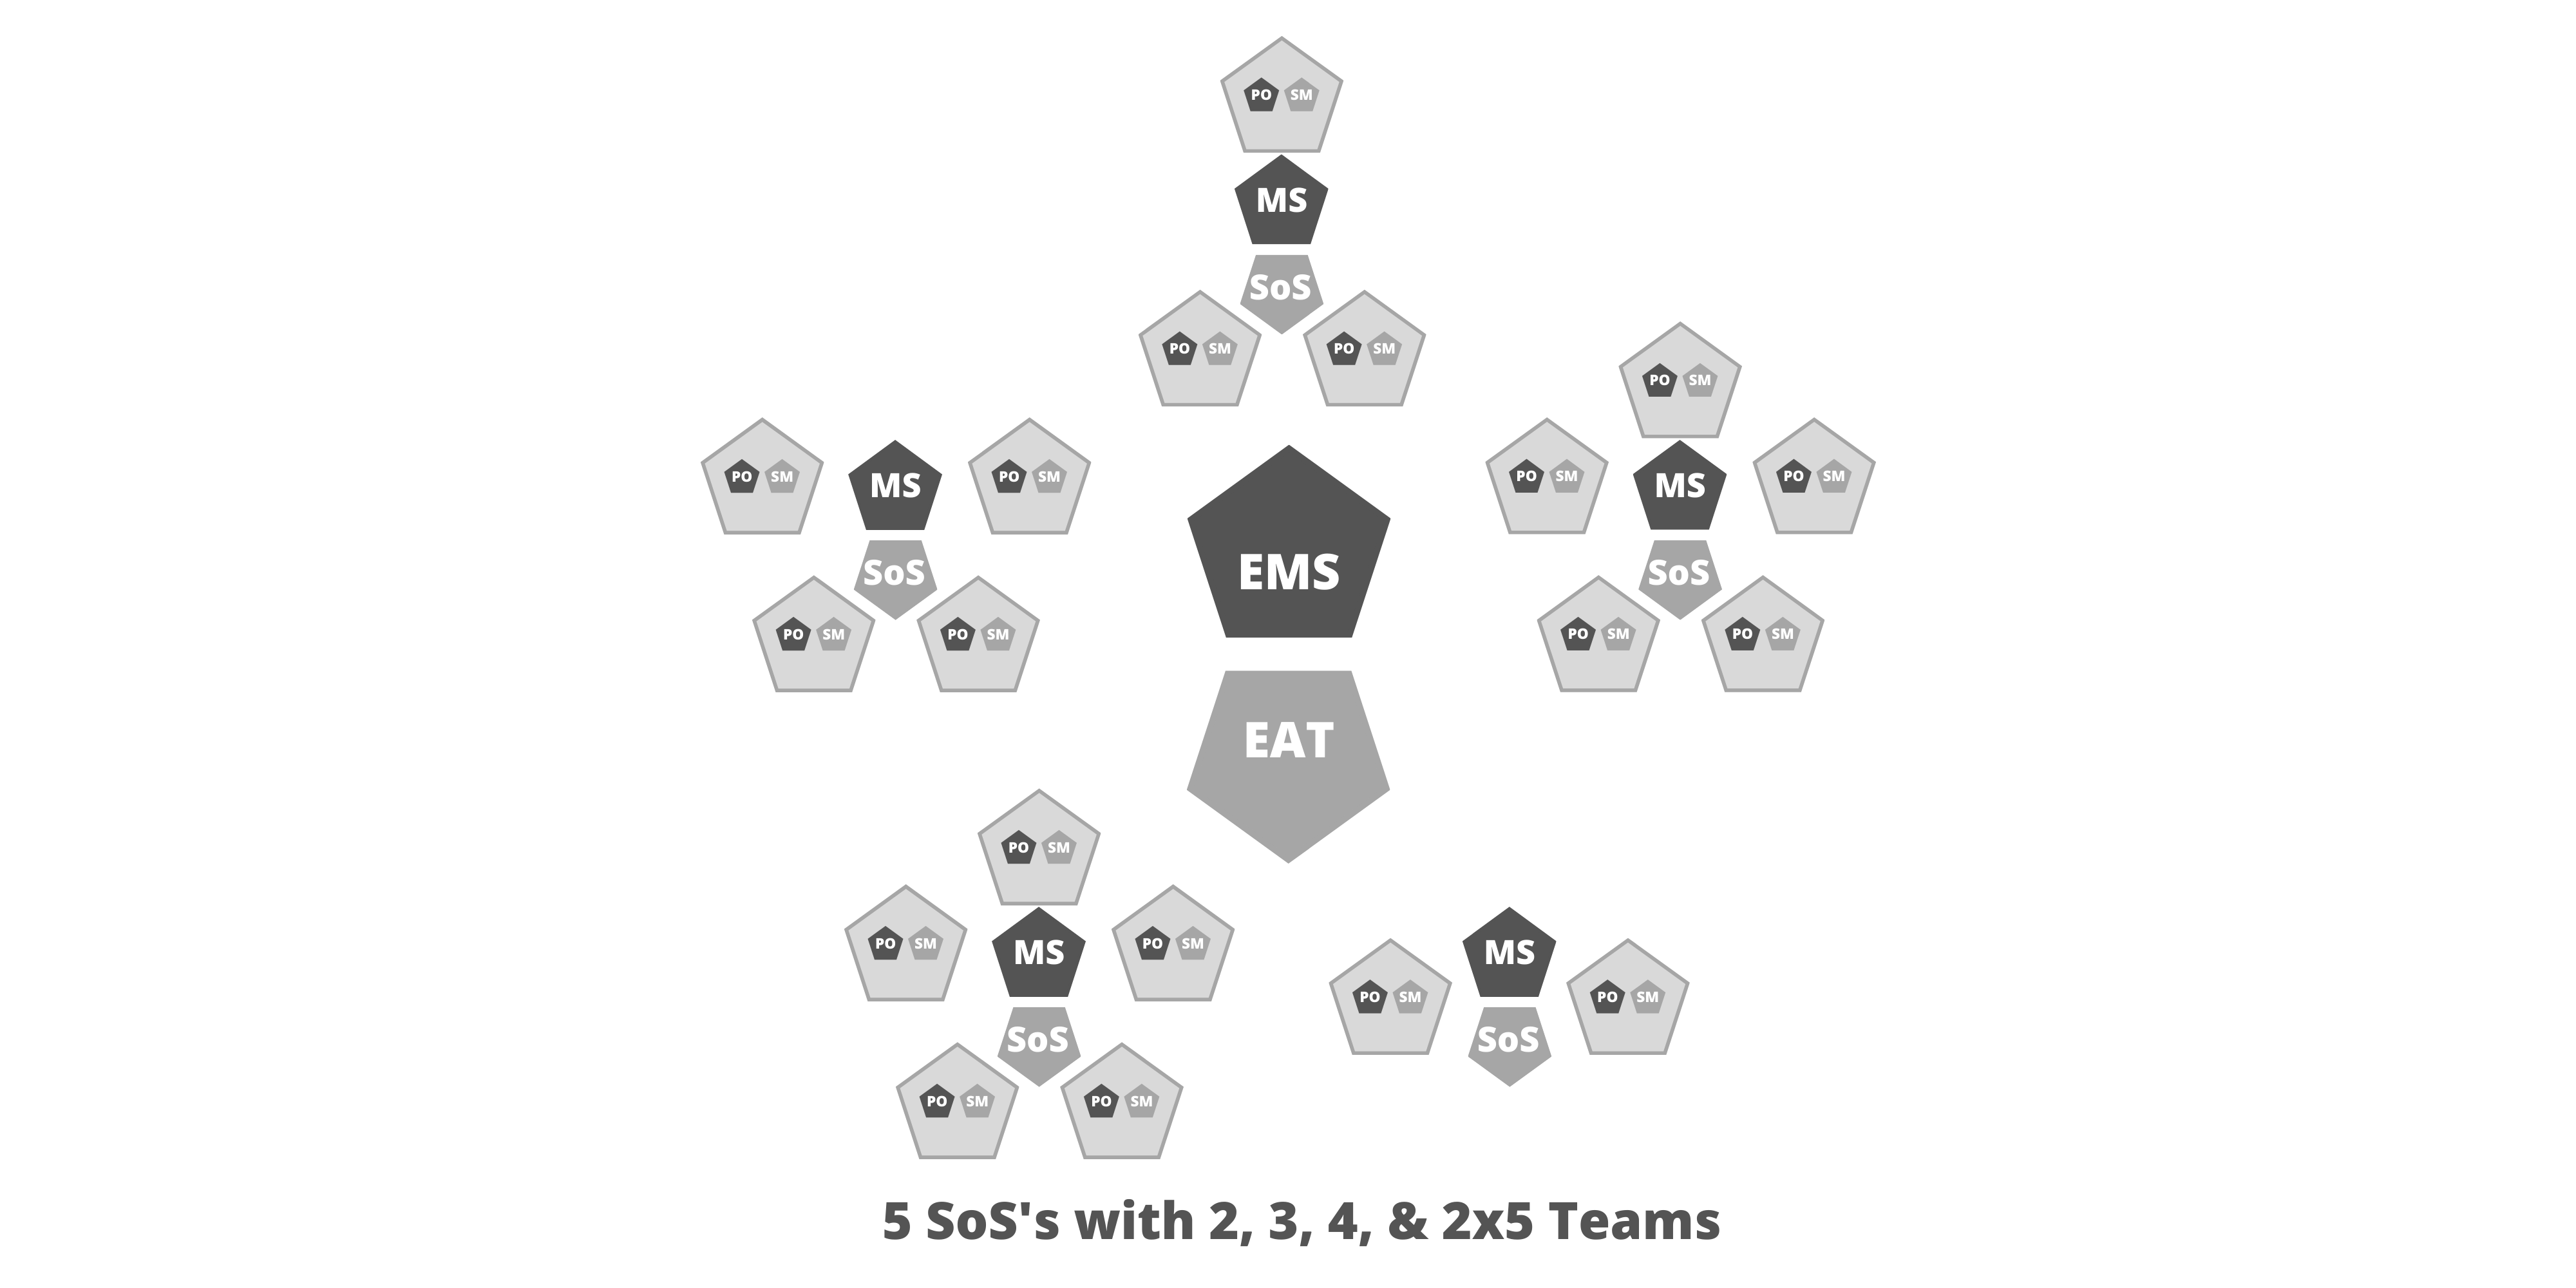
\includegraphics[scale=0.15]{4.png}
\end{figure}
\begin{figure}[H]
    \centering
    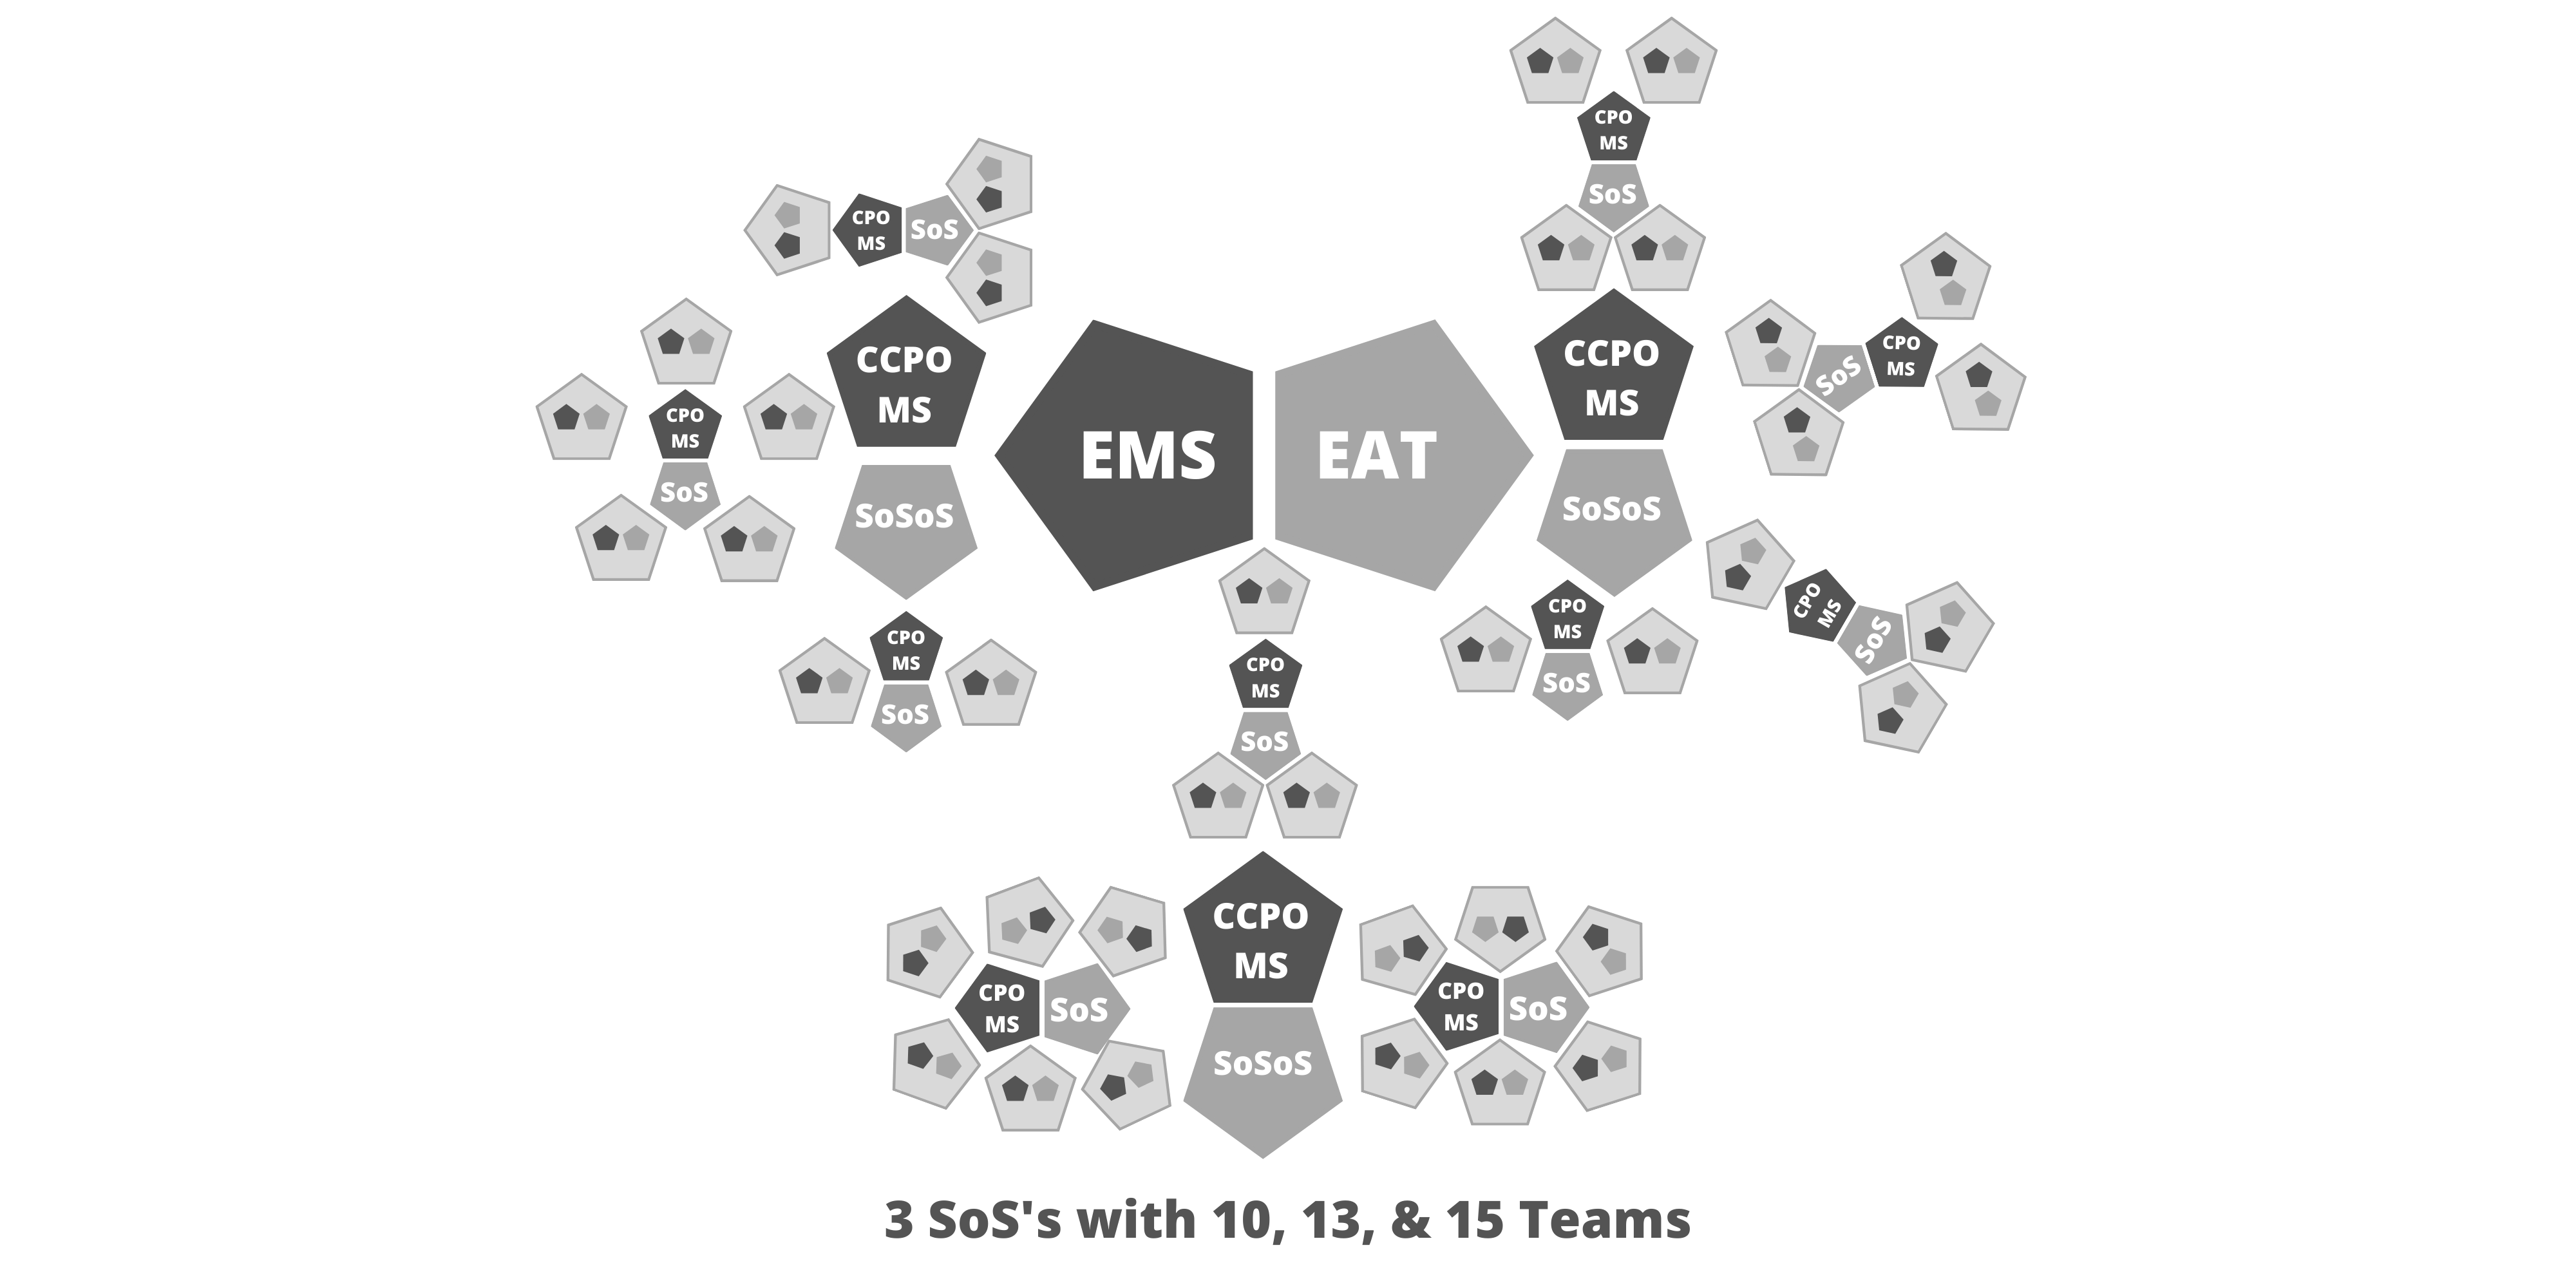
\includegraphics[scale=0.15]{5.png}
\end{figure}

Customer Relations, Legal / Compliance i~People Operations są tu uwzględnione, ponieważ są niezbędnymi częściami organizacji i~będą istnieć jako niezależne Scrum Teamy na własną rękę, na których mogą polegać wszystkie inne zespoły.

Ostatnia uwaga dotycząca przedstawicieli Executive Action Team i~Executive MetaScrum: Na tym diagramie są oni pokazani jako nakładający się, ponieważ niektórzy członkowie są częścią EAT i~uczestniczą w~wydarzeniu EMS. w~bardzo małych organizacjach lub implementacjach członkowie Executive Action Team i~uczestnicy wydarzenia Executive MetaScrum mogą składać się dokładnie z~tych samych osób.

\begin{figure}[H]
    \centering
    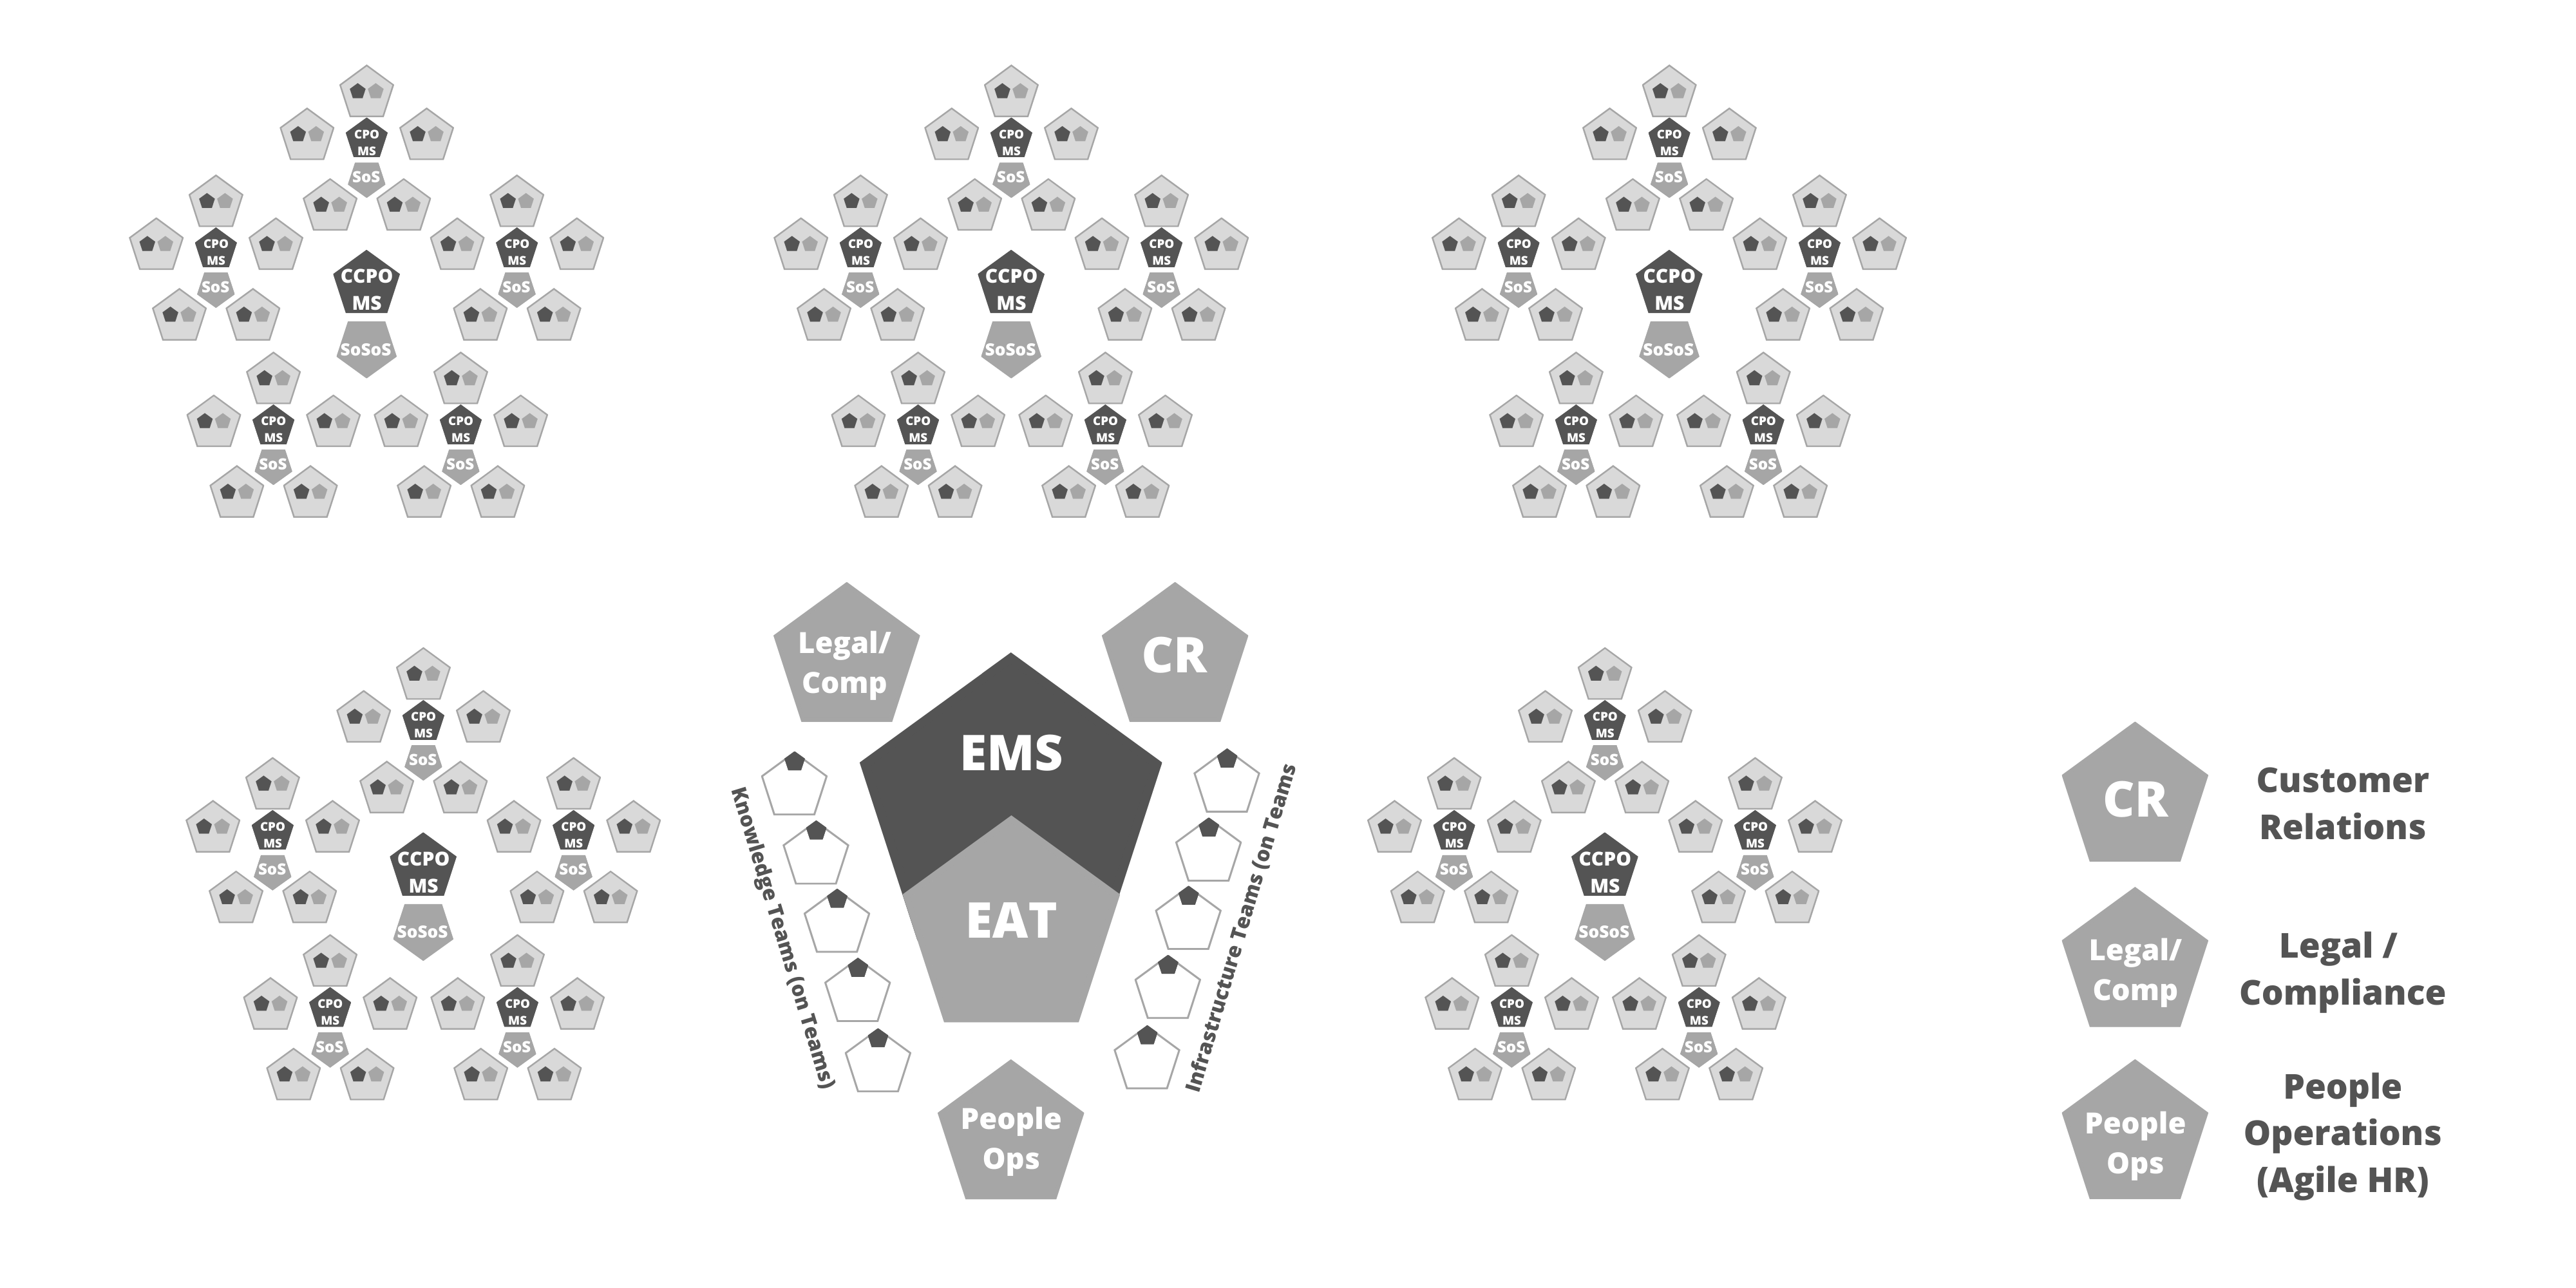
\includegraphics[scale=0.15]{6.png}
\end{figure}

\emph{W powyższym schemacie organizacyjnym, Knowledge Teams i~Infrastructure Teams reprezentują wirtualne zespoły specjalistów, których jest zbyt mało, aby obsadzić każdy z~nich. Jeśli działają one jako zespoły usług współdzielonych, koordynują swoje działania z~Scrum Teamami jako grupą, gdzie zapotrzebowanie przepływa przez Product Ownera dla każdej specjalności, który przekształca je w~transparentny backlog z~priorytetami. Ważną informacją jest to, że te zespoły NIE są silosami osób, które siedzą razem (dlatego są reprezentowane jako puste pięciokąty); członkowie ich zespołów siedzą w~rzeczywistych Scrum Teamach, ale tworzą ten wirtualny Scrum na własny użytek w~celu dzielenia się backlogiem i~poprawy procesu.}

\subsection{Nota końcowa}\label{End-Note}

Scrum@Scale został zaprojektowany do skalowania produktywności, tak aby cała organizacja dostarczała dwa razy więcej wartości przy połowie kosztów. Implementacja usprawnionego przepływu pracy w~stałym tempie, przy lepszym podejmowaniu decyzji, usprawnia środowisko pracy, zwiększa zwinność biznesową i~generuje wyższy zwrot dla wszystkich interesariuszy.

Scrum@Scale został zaprojektowany w~celu przesiąknięcia organizacji Scrumem. Dobrze zaimplementowany Scrum może uruchomić całą organizację z~Scrum@Scale jako systemem operacyjnym.

\subsection{Podziękowania}\label{Acknowledgements}

\subsubsection{Historia}\label{History}

Dr Jeff Sutherland opracował Scrum@Scale w~oparciu o~podstawowe zasady stojące za Scrum, teorię Złożonych Systemów Adaptacyjnych, teorię gier oraz swoją pracę w~biologii. Oryginalna wersja tego przewodnika powstała dzięki współpracy z~Jessicą Larsen, Avi Schneier i~Alexem Sutherlandem. Kolejne wydania zostały dopracowane dzięki wkładowi wielu doświadczonych praktyków Scruma w~oparciu o~wyniki ich pracy w~terenie.

\subsubsection{People and Organizations}\label{People-and-Organizations}

Wyrażamy uznanie dla IDX za stworzenie Scruma of Scrums, który jako pierwszy umożliwił skalowanie Scruma na setki zespołów\textsuperscript{\ref{6}}, PatientKeeper za stworzenie MetaScruma\textsuperscript{\ref{7}}, który umożliwił szybkie wdrożenie innowacyjnego produktu oraz OpenView Venture Partners za skalowanie Scruma na całą organizację. Cenimy wkład firmy Intel, która nauczyła nas, że ,,nic się nie skaluje poza architekturą bezskalową'', oraz firmy SAP, posiadającej największą organizację produktową z~Scrum Teamami, która nauczyła nas, że zaangażowanie managementu w~MetaScrum jest niezbędne, aby zebrać ponad 2000 Scrum Teamów do wspólnej pracy.

Trenerzy i~szkoleniowcy agile wdrażający te koncepcje w~Amazon, GE, 3M, Toyocie, Spotify, Maersk, Comcast, AT i~wielu innych firmach byli pomocni w~testowaniu tych koncepcji w~wielu firmach z~różnych dziedzin.

\subsection{Nota od tłumacza}

Podobnie jak Krystian Kaczor (tłumacz wersji 1.05 z~czerwca 2019) nie zdecydowałem się na tłumaczenie wszystkich pojęć, ale zachowałem wersje oryginalne tak, aby ułatwić zrozumienie i~odszukanie w~sieci. Dodatkowo pozostawiłem nieprzetłumaczone pojęcia, które funkcjonują w~innych, tłumaczonych przewodnikach, a~w~szczególności w~tłumaczeniu Przewodnika po Scrum. Zdecydowałem o~tym zdając sobie sprawę z~faktu, iż odbiorcami Przewodnika po Scrum@Scale są osoby z~doświadczeniem w~Scrum. 

Poniższe tłumaczenie jest całkowicie nowe, niezależne i~mam nadzieję, że przyniesie wielu osobom radość ze zrozumienia skalowania Scrum@Scale.

\subsubsection{Podziękowania}
\begin{itemize}
	\item Agile Coachowi (i~mojej żonie) - Izabeli Januszewskiej za wsparcie i~pomoc w~tłumaczeniu. Jej również dedykuję moją pracę włożoną w~tłumaczenie.
	\item ... oraz całemu środowisku zgromadzonemu wokół \href{https://www.agile.org.pl}{\underline{Stowarzyszenia Agile}}.
\end{itemize} 
Jeśli masz uwago do tłumaczenia lub widzisz możliwość jego poprawy nie wahaj sie napisać do mnie na adres \href{mailto:michal.januszewski@agile.org.pl}{\underline{michal.januszewski@agile.org.pl}}.

~
\pagebreak
\begin{center}\rule{3in}{0.4pt}\end{center}

\begin{enumerate}
\itemsep1pt\parskip0pt\parsep0pt
\item
  ``Business agility.'' Wikipedia, Last modified 27 February 2020.
  \newline ~\href{https://en.wikipedia.org/wiki/Business_agility}{https://en.wikipedia.org/wiki/Business\_agility}.
\item
  Johnson, Jim. New CHAOS Report. The Standish Group. 2018.
\item
  Ogunnaike, Babatunde A. and Ray, W. Harmon. Process Dynamics, Modeling and Control. Oxford University Press. 1994.
\item
  Hackman, J Richard. Leading Teams: Setting the Stage for Great Performances. Harvard Business Press. 2002.
\item
  \label{5} Sutherland, Jeff, Coplien, James O., and The Scrum Patterns Group. a~Scrum Book: The Spirit of the Game. Pragmatic Bookshelf. 2019.
\item
  \label{6} Sutherland, Jeff. ``Inventing and Reinventing SCRUM in five Companies.'' Sur le site officiel de l'alliance agile. 2001.
\item 
  \label{7} Sutherland, Jeff. ``Future of Scrum: Parallel Pipelining of Sprints in Complex Projects.'' Proceedings of the Agile Development Conference. IEEE Computer Society 90-102. 2005.
\item
  Sutherland, Jeff and Altman, Igor. ``Take No Prisoners: How a~Venture Capital Group Does Scrum.'' Agile Conference, 2009. AGILE'09, IEEE 350-355. 2009.
\end{enumerate}

\end{document}
